%%
% 今時jarticleやjbook使ってる人いる?時代はjsarticleかjsbookだよ
% ついでに言うと、uplatexってのはplatexの上位互換、これを使わないなんて旧世代だよね
%
\documentclass[uplatex, report, a4j, 10pt]{jsbook}


%%
% パッケージ群
%
\usepackage{packages/miyazaki-u-paper}   % 宮崎大学工学部の卒論の基本(片山先生作)を、僕がちょっと書き換えちゃった(テヘッ
\usepackage{enumitem}           % enumerate?古い古い
\usepackage[dvipdfmx]{graphicx} % 当然dvipdfmなんて使ってないよね
\usepackage[dvipdfmx]{color}    % listingsを使うときにはこれも必須、dvipdfmxを変えちゃうとgraphicxのdvipdfmxも変わるよ
\usepackage{listings, packages/jlisting} % コードを埋め込むなら必須
\lstset{
	label={some_label}
    backgroundcolor=\color{lightgray},
    basicstyle=\ttfamily\small,
    breaklines=true,
    showstringspaces=false
}
\usepackage{txfonts}            % フォントといえばやっぱりtxfonts、今はnewtxってのもあるらしい
\usepackage{verbatim}           % コメントアウトしてくれる便利なプリアンブルが使える \begin{comment} ... \end{comment}
\usepackage{url}
% \usepackage{easy-todo}
\usepackage[hdivide={21mm, , 21mm}, vdivide={30mm, , 25mm}]{geometry} % スタイルを少し変えたくても\hoffset, \voffsetは使わないでね
\usepackage{multirow}
\usepackage{ascmac}


% \usepackage{latexsym}
% \usepackage{bmpsize}
% \usepackage{comment}

% \def\Underline{\setbox0\hbox\bgroup\let\\\endUnderline}
% \def\endUnderline{\vphantom{y}\egroup\smash{\underline{\box0}}\\}

\newcommand{\ttt}[1]{\texttt{#1}}
\newcommand{\toolName}{MixVRT}  % ツール名を設定

%%
% miyazaki-u-paper.sty用設定値
%
\degree{g} % Graduateのg or Masterのm
\figurenumbering{f} % 図目次を付ける場合はt (真) を持つ真偽値を引数に取る関数
\tablenumbering{f} % 表目次を付ける場合はt (真) を持つ真偽値を引数に取る関数
\title{Webページの画像とHTMLコードにおける\\レイアウトの不具合箇所可視化を目的とした\\視覚的回帰テスト支援ツールMixVRTの試作}
\author{有留 直希}
\nendo{5} % 年度
\advisor{片山 徹郎 教授} % 修論では無視する
\major{情報システム工学科}


\begin{document}
\maketitle

%
% 概要
% 
\preface{概要}
ここに概要を書く。


%
% 本文
% 
\chapter{はじめに}\label{cha:Introduction}

最初に、目視で変更前後のWebページを見比べて、不具合がないかどうかを見つけることの難しさを記述する。
\begin{itemize}
    \item Item 01
    \item Item 02
    \item Item 03
\end{itemize}

画像ベースの視覚的回帰テストの説明と、その問題点について記述する。
\begin{itemize}
    \item Item 01
    \item Item 02
    \item Item 03
\end{itemize}

本研究で試作するツールで課題を解決できることについて記述する。
\begin{itemize}
    \item Item 01
    \item Item 02
    \item Item 03
\end{itemize}

\par
本論文の構成を、以下に示す。\par
第2章では、本研究に必要となる前提知識を説明する。\par
第3章では、MixVRTの機能と外観について説明する。\par
第4章では、MixVRTの実装について説明する。\par
第5章では、適用例を用いて、MixVRTが正しく動作することを示す。\par
第6章では、MixVRTについて考察する。\par
第7章では、本研究のまとめと今後の課題について述べる。



% \begin{figure}[t]
%     \begin{center}
%         \includegraphics[width=7cm]{image/sample.png}
%         \caption{sample image}
%         \label{fig:sample}
%     \end{center}
% \end{figure}
\chapter{研究の準備}\label{cha:Preparation}

\section{視覚的回帰テスト}\label{sec:vrt}
視覚的回帰テスト (Visual regression testing)\cite{Visual regression testing}は、
Webページの変更前画像と変更後画像を比較し差分を検出することで、意図しないレイアウトの変更が発生していないことを確認するテスト手法である。\\
視覚的回帰テストの基本的な手順は以下の通りである。
\begin{enumerate}
      \setlength{\itemsep}{0pt}
            \setlength{\parsep}{0pt}
      \item 変更前画像と変更後画像の作成
      \item 画像比較による差分検出
      \item 結果の評価
\end{enumerate}

\section{レイアウトの不具合}\label{sec:layout effect}
レイアウトの不具合は、Webページの画面要素(テキストやボタン、画像など)が適切にレイアウトされていないことである。
【TODO: レイアウトの不具合検出に関する関連研究のリンクを見つける】
\par
本研究では、以下の主な3つのレイアウトの不具合を検出する。
\begin{itemize}
      \setlength{\itemsep}{0pt}
            \setlength{\parsep}{0pt}
      \item 画面要素の隠れ:\\
            Webページの画面要素がその画面要素を含むコンテナやビューポートの境界を超えてはみ出している状態。
      \item 画面要素の見切れ:\\
            Webページの画面要素の一部がコンテナやビューポートの境界によって切り取られ、完全には表示されない状態。
      \item 画面要素の重なり:\\
            Webページの複数の画面要素が重なりあっている状態。
\end{itemize}
% また、以下の画面要素に対して、レイアウトの不具合を検出する。
% \begin{itemize}
%     \setlength{\itemsep}{0pt}
%           \setlength{\parsep}{0pt}
%     \item テキスト
%     \item 画像
%     \item ボタン
%     \item ヘッダー
%     \item フッター
% \end{itemize}

\section{OpenCV}\label{sec:opencv}
OpenCV (Open Source Computer Vision Library)は、画像や動画に関する処理機能をまとめた、コンピュータビジョン向けのオープンソースのライブラリである\cite{OpenCV}。
\par
本研究では、OpenCVに用意されている、imread関数、cvtColor関数、adaptiveThreshold関数、subtract関数、findContours関数、boundingRect関数、rectangle関数、absdiff関数の8つの関数を用いる。
\paragraph{imread関数}
imread関数は、画像ファイルの読み込みを行う関数である。
第一引数に、画像ファイルのパスを指定する。
\paragraph{cvtColor関数}
cvtColor関数は、画像の色空間を変換する関数である。
第一引数には、色空間の変換を適用する画像を指定し、第二引数には、どの色空間へ変換するかを示すコード(例: cv2.COLOR\_BGR2GRAY、cv2.COLOR\_GRAY2BGR)を指定する。
\par
本研究では、BGR(青、緑、赤)からGRAY(グレースケール)と、GRAY(グレースケール)からBGR(青、緑、赤)の色空間への変換に用いる。
\paragraph{adaptiveThreshold関数}
adaptiveThreshold関数は、画像の各小領域(画像を複数の小さな区画に切り分けた各々の部分)ごとに異なる二値化の閾値を用いて画像の二値化を行う関数である。
第一引数には、二値化を適用するグレースケール画像を指定し、第二引数には、二値化後のピクセル最大値(通常$255$)を指定する。
第三引数には、二値化の閾値を計算する方法を指定し、第四引数には、二値化の方法を指定する。
第五引数には、近傍領域(特定のピクセルを中心とした周囲のピクセルの集合)のサイズ(例: 3 $\times$ 3ピクセルの正方形)を指定し、
第六引数には計算された二値化の閾値から引かれる定数を指定する。
\par
本研究において、adaptiveThreshold関数の引数に指定するパラメータを、以下に示す。
\begin{itemize}
      \setlength{\itemsep}{0pt}
            \setlength{\parsep}{0pt}
      \item 二値化の閾値を計算する方法:\\
            近傍領域内のピクセル平均値(近傍領域内のピクセル合計値 $\div$ 近傍領域内のピクセル数)に基づいて閾値を計算するcv2.ADAPTIVE\_THRESH\_MEAN\_Cを用いる。
      \item 二値化の方法:\\
            二値化の閾値以下のピクセル値をピクセル最大値($255$)に変換し、
            それ以外のピクセル値を$0$に変換する二値化方法であるcv2.THRESH\_BINARY\_INVを用いる。
      \item 近傍領域のサイズ:\\
            $11$(11 $\times$ 11ピクセルの正方形)に設定する。
      \item 計算された二値化の閾値から引かれる定数:\\
            $2$に設定する。
\end{itemize}
\par
また、本研究におけるadaptiveThreshold関数は、画像の一部が明るく、他の部分が暗い場合においても、全体として均一な白黒画像を生成するために用いる。
% \paragraph{bitwise\_not関数}
% bitwise\_not関数は、画像の各ピクセル値のビットを反転する関数である。
% ビット反転の例として、黒ピクセル($0$のピクセル値)は白ピクセルに(ピクセル値が$255$に)、白ピクセル($255$のピクセル値)は黒ピクセルに(ピクセル値が$0$に)反転する。
% 第一引数にビット反転を行う画像を指定する。
\par
\paragraph{subtract関数}
subtract関数は、2つの画像間の対応するピクセル値を比較し、差を計算する関数である。差を計算した結果の画像を返す。
第一引数には、比較の基準となる画像を指定する。この画像の各ピクセル値から、第二引数で指定する画像の対応するピクセル値を引く。
第二引数には、第一引数の画像と比較する画像を指定する。この画像の各ピクセル値が、第一引数で指定する画像の対応するピクセル値から引かれる。
\par
subtract関数の適用例として、
第一引数に二値化画像Aを、第二引数に二値化画像Bを指定すると、二値化画像Aにのみ存在する白ピクセル領域を抽出した差分画像を生成する。
なお、二値化画像AとBはそれぞれ白ピクセル領域に特徴がある画像(例: 二値化前の画像AとBが元々Webページの画像であり、Webページ内のテキストやボタンなどの画面要素が二値化後の画像で白ピクセル領域、それ以外の背景などが黒ピクセル領域となっている画像)とする。
\par
二値化画像AとB間で対応するピクセル値の差を計算する処理を、以下に示す。
\begin{itemize}
      \setlength{\itemsep}{0pt}
            \setlength{\parsep}{0pt}
      \item 共通の白ピクセル(AとB両方で白):\\
            二値化画像AとBの両方で白ピクセルの場合、subtract関数は$255$(Aの白ピクセル値)から$255$(Bの白ピクセル値)を引く。
            差は$0$(黒ピクセル値)になり、共通の白ピクセルは黒ピクセルとなる。
      \item Aにのみ存在する白ピクセル(Aは白、Bは黒):\\
            画像Aは白ピクセルで、画像Bは黒ピクセル(ピクセル値が$0$)の場合、subtract関数は$255$(Aの白ピクセル値)から$0$(Bの黒ピクセル値)を引く。
            差は$255$(白ピクセル値)になり、Aにのみ存在する白ピクセルはそのまま残る。
      \item Bにのみ存在する白ピクセル(Aは黒、Bは白):\\
            画像Aは黒ピクセルで、画像Bは白ピクセルの場合、subtract関数は$0$(Aの黒ピクセル値)から$255$(Bの白ピクセル値)を引く。
            差は$-255$になるが、subtract関数は負の値を$0$(黒ピクセル値)として処理するため、Bにのみ存在する白ピクセルは黒ピクセルとなる。
\end{itemize}
上記の処理の結果、二値化画像Aにのみ存在する白ピクセル領域を抽出した差分画像を生成する。
\par
本研究では、二値化処理を行った、Webページの変更前画像と変更後画像をそれぞれ交互に1回ずつsubtract関数の第一引数と第二引数に指定し実行することで、
変更前画像から削除された箇所を抽出した差分画像と、変更後画像に追加された箇所を抽出した差分画像を生成する。
\paragraph{dilate関数}
dilate関数は、二値化画像内の白ピクセル領域を拡大する(膨張処理を行う)関数であり、ノイズ除去やオブジェクトの形状とサイズの強調に役立つ。
カーネルと呼ばれる特定の形状とサイズの小さなフィルタを使用し、フィルタを画像上でスライドし各ピクセルに対して、
フィルタ内の最大値をそのピクセルに割り当てていくことで、白ピクセル領域を拡大する。
第一引数に、膨張処理を行う画像を指定する。
第二引数に、カーネルのサイズと形状を指定する。
第三引数に、膨張処理の適用回数を指定する。
\par
本研究において、adaptiveThreshold関数の引数に指定するパラメータを、以下に示す。
\begin{itemize}
      \setlength{\itemsep}{0pt}
            \setlength{\parsep}{0pt}
      \item カーネルのサイズと形状:\\
            5 $\times$ 5ピクセルの正方形に設定する。
      \item 膨張処理の適用回数:\\
            $6$に設定する。
\end{itemize}
\par
また、本研究におけるdilate関数は、subtract関数で抽出した、削除された箇所と追加された箇所の形状とサイズを強調することで、
影響箇所(\ref{cha:Function}章で後述)を枠で囲む粒度と同じ程度の粒度で、
後述するrectangle関数が削除された箇所と追加された箇所を枠で囲むことを目的としている。
この目的の結果、レイアウトの不具合箇所(\ref{cha:Function}章で後述)の検出精度を高めることができる。
% 差分箇所(\ref{cha:Function}章で後述)を枠で囲む粒度を、影響箇所(\ref{cha:Function}章で後述)を枠で囲む粒度に近づけることができるため、
% レイアウトの不具合箇所の検出に役立つ。
% 本研究では、差分箇所を枠で囲む粒度を、影響箇所を枠で囲む粒度と合わせるために用いる。
\paragraph{findContours関数}
findContours関数は、画像から輪郭を検出し、輪郭リストを返す。
第一引数に輪郭抽出する画像(通常は二値化画像)を指定する。
第二引数に輪郭構造の取得方法を指定する。
第三引数に、輪郭座標の取得方法を指定する。
\par
本研究において、findContours関数の引数に指定するパラメータを、以下に示す。
\begin{itemize}
      \setlength{\itemsep}{0pt}
            \setlength{\parsep}{0pt}
      \item 輪郭構造の取得方法:\\
            画像内の一番外側の白の輪郭のみを取得するRETR\_EXTERNALを用いる。
      \item 輪郭の形成方法:\\
            端点のみで輪郭を形成するCHAIN\_APPROX\_SIMPLEを用いる。
\end{itemize}
\par
また、本研究におけるfindContours関数は、
Webページの変更前画像から削除された箇所を抽出し膨張処理を行った差分画像から、削除された箇所の輪郭座標を、
Webページの変更後画像に追加された箇所を抽出し膨張処理を行った差分画像から、追加された箇所の輪郭座標を取得するために用いる。
\paragraph{boundingRect関数}
boundingRect関数は、輪郭データにもとに、その輪郭を完全に囲む最小の矩形(バウンディングボックス)を計算する関数である。
第一引数は、findContours関数で取得した輪郭リストの各要素である輪郭データを指定する。
なお、輪郭データは、単一の輪郭を表す配列であり、この配列に輪郭を形成する点の集合を含む。
\par
本研究におけるboundingRect関数は、矩形の左上の点のx座標とy座標、さらに矩形の幅と高さを取得するために用いる。
これにより、輪郭を取り囲む矩形の位置とサイズを取得できる。
\paragraph{rectangle関数}
rectangle関数は、画像に矩形を描画する関数である。
第一引数に描画先の画像、第二引数に矩形の左上の点の座標、第三引数に矩形の右下の点の座標、
第四引数に矩形の色、第五引数に矩形の線の太さを指定する。
\par
本研究におけるrectangle関数は、画像上に指定された位置と大きさの矩形を指定された色で描画し、特定の領域を視覚的に強調するために用いる。
\paragraph{absdiff関数}
absdiff関数は、2つの配列または画像間の絶対値の差を計算する関数である。
第一引数に、第一の入力配列または画像を指定する。この配列または画像のデータ型は、第二の入力配列または画像と一致している必要がある。
第二引数に、第二の入力配列または画像を指定する。この配列または画像は、第一の入力配列または画像と同じサイズとデータ型である必要がある。
\par
本研究におけるabsdiff関数は、入力された2つの配列または画像の各ピクセル値の絶対差を計算し、その結果を出力配列または画像として返す。
具体的には、absdiff(src1, src2)は、src1とsrc2の各ピクセルについて$|src1 - src2|$の計算を行い、その結果を新しい画像として出力する。

\section{Pillow}\label{sec:pillow}
Pillow\cite{Pillow}は、Python\cite{Python}の画像処理ライブラリの1つで、画像の読み込み、処理、保存などの機能を提供する。
本研究では、Pillowに用意されている、Image.open関数、Image.LANCZOSを用いる。
\paragraph{Image.open関数}
Image.open関数は、指定したパスの画像ファイルを開き、PillowライブラリによるImageクラスのインスタンスを生成して返す。
このImageクラスのインスタンスでは、画像のサイズ変更、回転、色調整など、様々な画像処理操作が可能である。
\paragraph{Image.LANCZOS}
Image.LANCZOSは、画像のサイズ変更時に使用されるリサンプリングフィルタ(アルゴリズム)の1つである\cite{LANCZOS}。
LANCZOSフィルタは、画像を拡大する際に細部やエッジを維持できるため、高解像度画像の生成処理に適している。

\section{Selenium WebDriver}\label{sec:Selenium_WebDriver}
Selenium WebDriver\cite{Selenium WebDriver}は、Seleniumプロジェクト\cite{Selenium}の一部であり、Webブラウザを直接制御するためのAPIを提供する。
Selenium WebDriverのAPIを用いてテストスクリプトを実行することで、指定したWebページにアクセスし、要素のクリックやページ遷移などのユーザ操作を自動で行う。

\section{requestsモジュール}\label{sec:requests}

\section{difflibモジュール}\label{sec:difflib}

\section{Flask}\label{sec:Flask}
Flask\cite{Flask}は、Pythonで構築されたWebフレームワークであり、WebサーバやWebアプリケーションの構築を容易にする。
このフレームワークは、Werkzeug\cite{Werkzeug}とJinja2\cite{Jinja}に基づいている。
WerkzeugはWebサーバとWebアプリケーション間のリクエストやレスポンスを処理するWSGIツールキットで、
WSGI(Web Server Gateway Interface)\cite{WSGI}はWebサーバとWebアプリケーション間の接続規格である。
Jinja2は、Pythonで使用されるテンプレートエンジンで、Webページの動的なレンダリングを可能にする。
\par
本研究では、Flaskを用いてローカルサーバを構築し、以下を実現する。
\begin{itemize}
      \setlength{\itemsep}{0pt}
            \setlength{\parsep}{0pt}
      \item \toolName による視覚的回帰テストで生成した画像(\ref{subsec:MixVRT_IO}節で後述)の確認が効率的に行えるWebページを開発者に提供する。
      \item HTML比較部(\ref{sec:Affected_area_extraction}節で後述)で生成した枠付きHTMLコードをレンダリングし、
            Flaskを用いて定義した特定のURLへのアクセスを通じて、レンダリングを行った枠付きWebページを表示する。
\end{itemize}
なお、枠付きWebページを表示する目的は、Selenium WebDriverを用いた、枠付きWebページの画像取得を可能にするためである。

\section{\toolName の環境構築}\label{sec:MixVRT_env_gen}
\toolName の環境構築には、ローカルサーバ用、Python処理用、およびSeleniumのChrome用の、合計3つのDockerコンテナ\cite{Docker Container}を使用する。
Docker Compose\cite{Docker Compose}を用いて、開発者はこれらのコンテナを同時に起動する。
ローカルサーバ用コンテナは、flaskを用いたローカルサーバを提供する。
Python処理用コンテナは、Pythonを用いた画像処理やHTMLコード解析処理を行う。
SeleniumのChrome用コンテナは、Webブラウザの自動操作を実行するためのChrome環境を提供する。
なお、これらのコンテナに必要な設定と依存関係は、Dockerfileとdocker-compose.ymlに定義している。
Dockerfileは、Dockerコンテナの構築に必要な指示を記述したファイルである。
docker-compose.ymlは、複数のコンテナを管理するための設定ファイルである。
\chapter{ \toolName の外観と機能}\label{cha:Function}
本章では、本研究で試作したツール\toolName (Mix Visual Regression Test)の外観と機能について説明する。
\par
\toolName は、レイアウトの不具合の発見を支援する、視覚的回帰テスト支援ツールである。
WebページのURLを入力とし、Webページの画像とHTMLコードに基づいてレイアウトの不具合を含む可能性がある箇所を可視化した、
インターフェース(レイアウトの不具合確認画面ビュー)を出力する。【TODO: これを出力することでこういうことが分かるというのを考える。そうすればおのずと出力するものが分かるはず】
\par
\toolName の外観を、図\ref{fig: Appearance}に示す。
\begin{figure}[tp]
    \begin{center}
        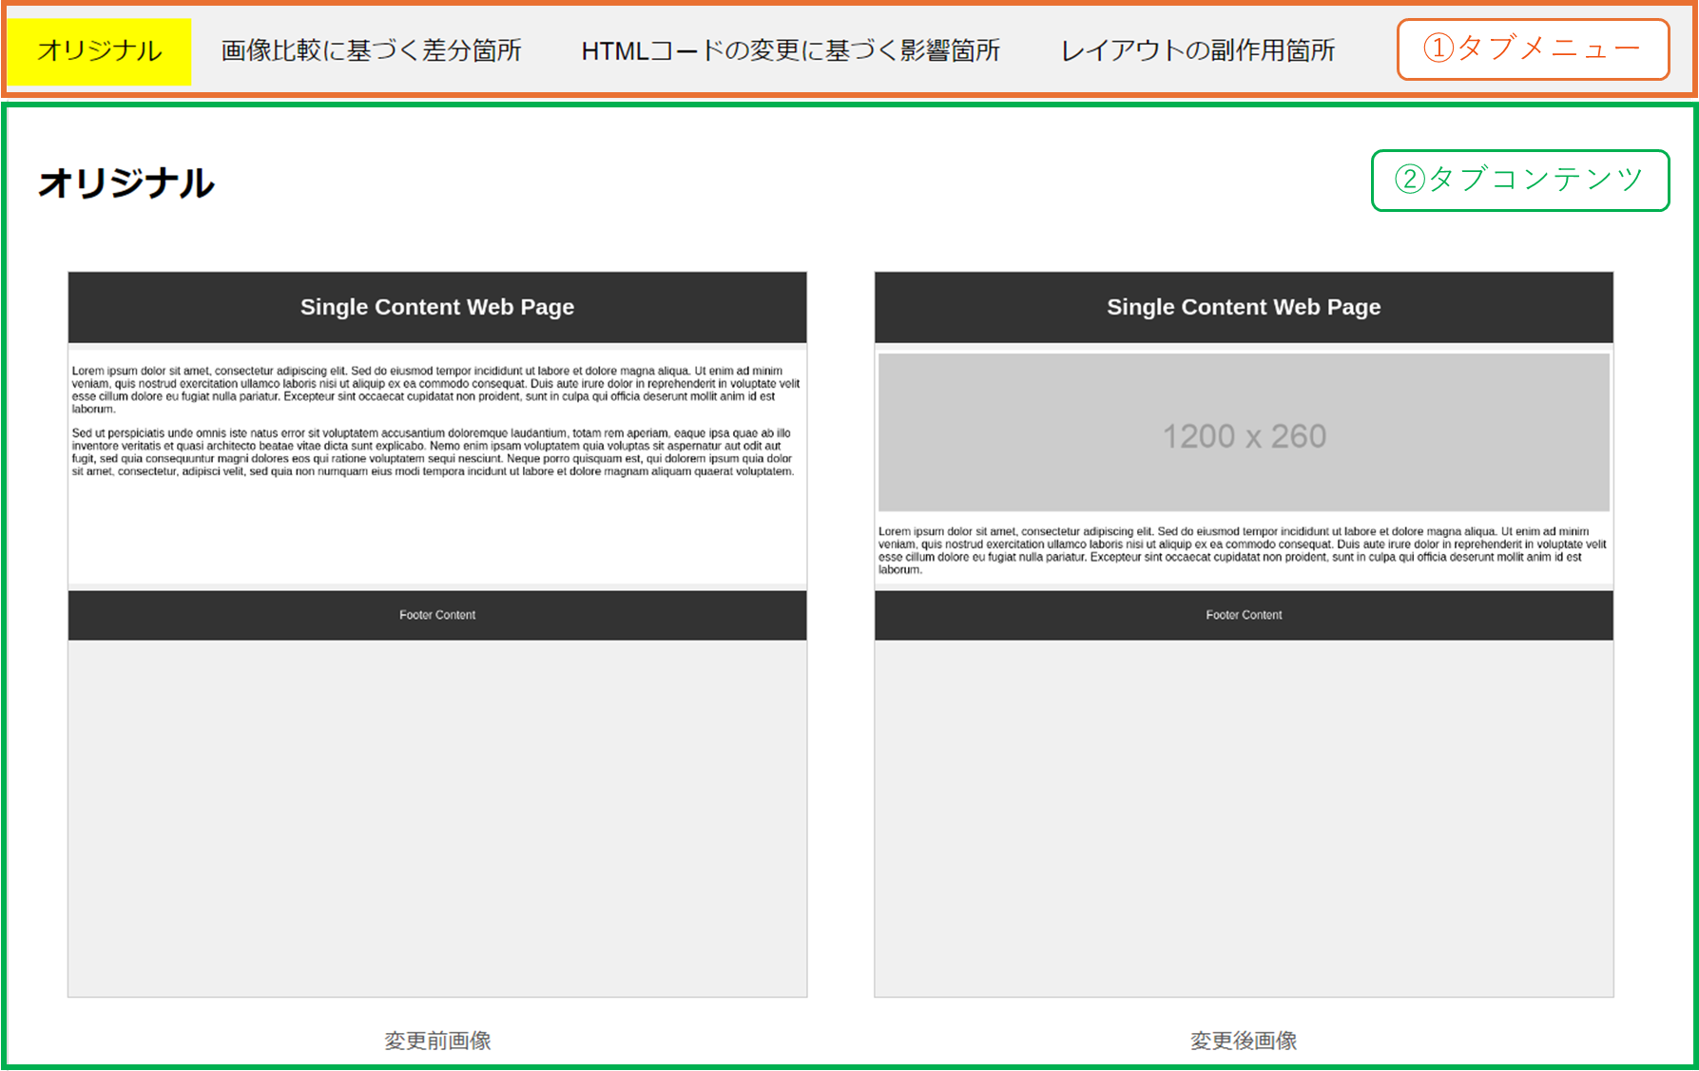
\includegraphics[width=1.0\columnwidth]{image/3_Outline_Appearance.png}
        \caption{\toolName の外観}
        \label{fig: Appearance}
    \end{center}
\end{figure}
% \toolName は、以下に示す4つのタブからなるタブメニューと各タブに対応した内容を表示するタブコンテンツからなる。
% なお、以下の数字は、図\ref{fig: Appearance}の数字と対応している。
% \begin{itemize}
%     \item タブメニュー
%     \item タブコンテンツ
% \end{itemize}
% \par
% また、タブメニューを構成する4つのタブは以下の通りである。
% \begin{itemize}
%     \item [①]オリジナル画像表示タブ
%     \item [②]画像比較に基づく差分箇所表示タブ
%     \item [③]HTMLコードの変更に基づく影響箇所表示タブ
%     \item [④]レイアウトの副作用箇所表示タブ
% \end{itemize}
% \par
% 以降、各タブの外観と機能について説明する。
% Webアプリケーションとして試作した\toolName は、以下に示す4つのタブからなるタブメニューと各タブに対応した内容を表示するタブコンテンツからなる。
% なお、以下の数字は、図\ref{fig: Appearance}の数字と対応している。
\toolName は、以下に示す4つのタブからなるタブメニューと各タブに対応した内容を表示するタブコンテンツからなる。
なお、以下の数字は、図\ref{fig: Appearance}の数字と対応している。
\begin{itemize}
    \item[①] タブメニュー
          \begin{itemize}
              \item オリジナル表示タブ
              \item 画像比較に基づく差分箇所表示タブ
              \item HTMLコードの変更に基づく影響箇所表示タブ
              \item レイアウトの副作用箇所表示タブ
          \end{itemize}
    \item[②] タブコンテンツ
\end{itemize}
\par
以降、各タブの外観と機能について説明する。



\section{オリジナル表示タブ}\label{subsec:original_tab}
オリジナル表示タブを押すと、Webページの変更前画像とWebページの変更後画像を表示する。
オリジナル表示タブを押した際の\toolName の画面例を、図\ref{fig: Appearance_original_tab}に示す。
なお、\toolName に一番最初にアクセスした時やリロードした時に、デフォルトでオリジナル表示タブを選択した状態になっている。
このタブでは、【TODO: ここでの目的を具体的に記述する】Webページの変更前後の画像を目視で確認できる。
\begin{figure}[tp]
    \begin{center}
        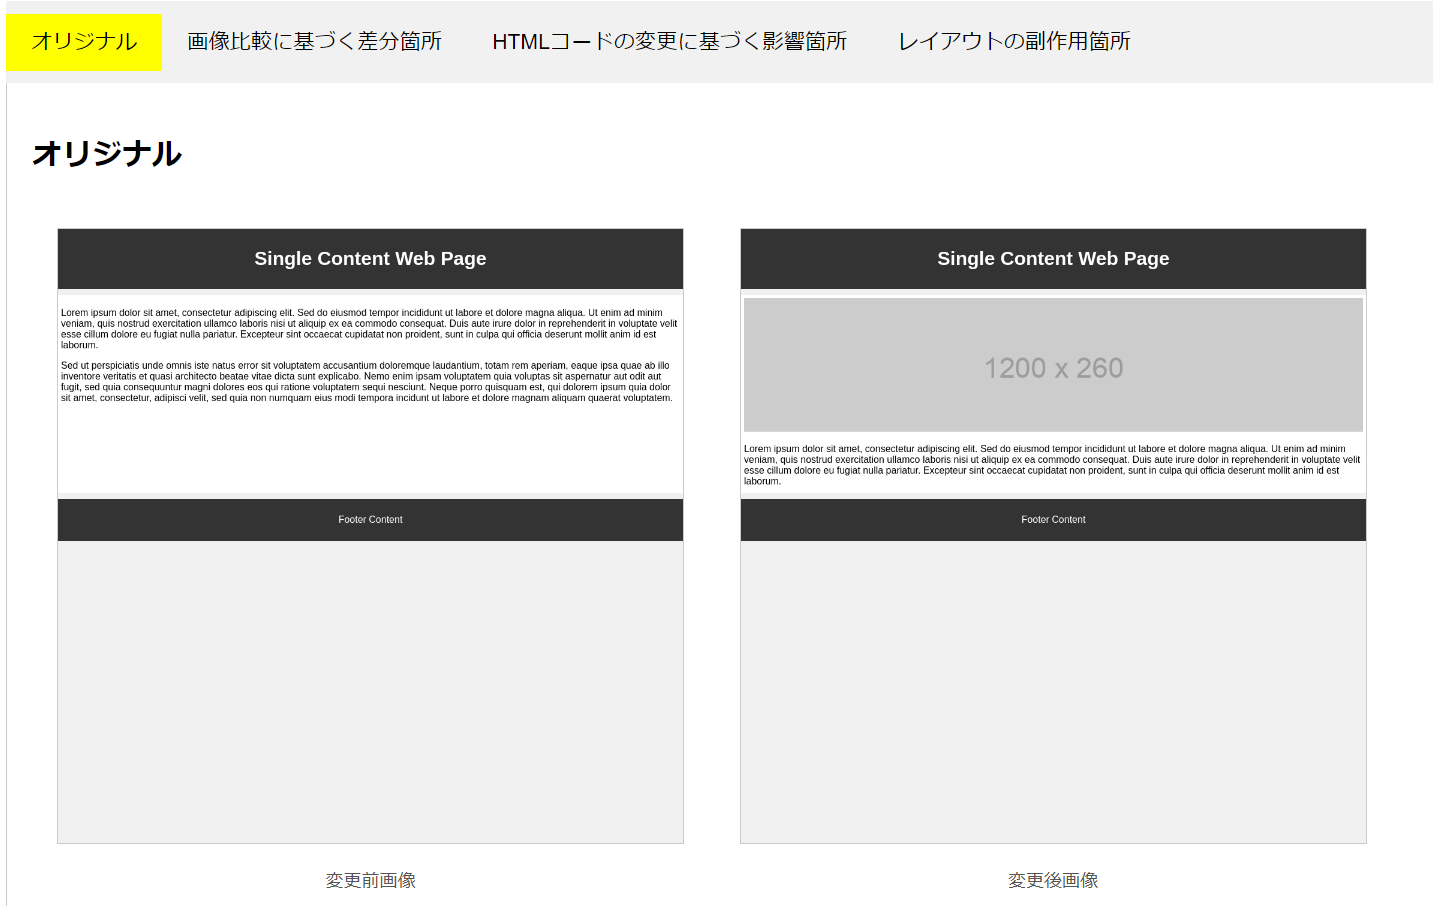
\includegraphics[width=1.0\columnwidth]{image/3_original_tab.png}
        \caption{オリジナル表示タブを押した際の\toolName の画面例}
        \label{fig: Appearance_original_tab}
    \end{center}
\end{figure}



\section{画像比較に基づく差分箇所表示タブ}\label{subsec:images_tab}
画像比較に基づく差分箇所表示タブを押すと、画像比較に基づく差分箇所を色付きの枠で囲んで強調表示した、Webページの変更前画像とWebページの変更後画像を表示する。
画像比較に基づく差分箇所表示タブを押した際の\toolName の画面例を、図\ref{fig: Appearance_images_tab}に示す。
ここでの差分箇所とは、変更前後のWebページを比較して、変更前のWebページで削除された箇所と変更後のWebページで追加された箇所を差分箇所と定義する。
削除された箇所は変更前画像上に赤枠で囲んで強調表示し、追加された箇所は変更後画像上に緑枠で囲んで強調表示する。
このタブでは、変更前後のWebページで画像比較によって差分が出た箇所を目視で確認できる。
\begin{figure}[tp]
    \begin{center}
        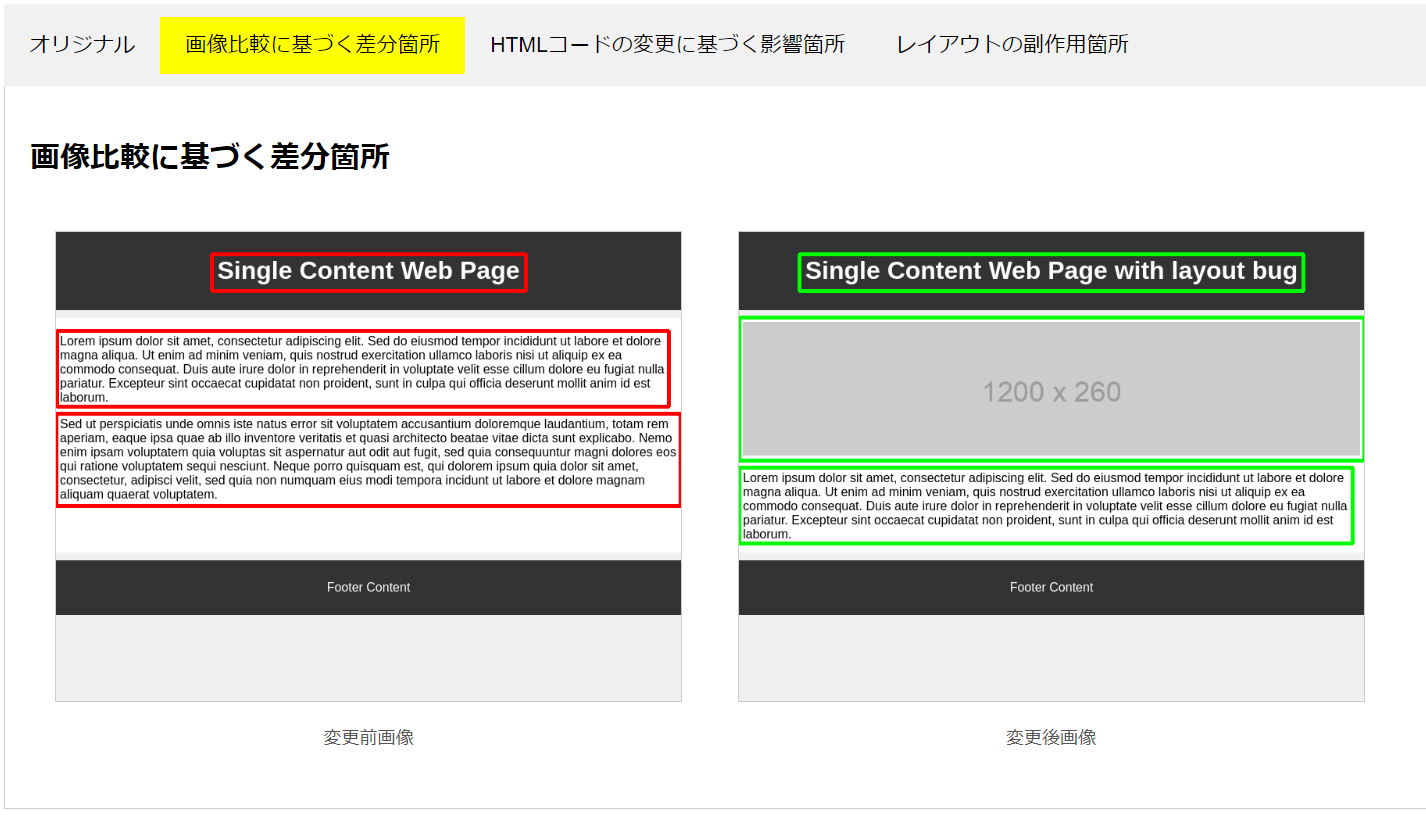
\includegraphics[width=1.0\columnwidth]{image/3_images_tab.png}
        \caption{画像比較に基づく差分箇所表示タブを押した際の\toolName の画面例}
        \label{fig: Appearance_images_tab}
    \end{center}
\end{figure}



\section{HTMLコードの変更に基づく影響箇所表示タブ}\label{subsec:html_tab}
HTMLの変更に基づく影響箇所表示タブを押すと、HTMLの変更に基づく影響箇所を色付きの枠で囲んで強調表示した、Webページの変更前画像とWebページの変更後画像を表示する。
HTMLの変更に基づく影響箇所表示タブを押した際の画面例を、図\ref{fig: Appearance_html_tab}に示す。
ここでの影響箇所とは、変更前後のWebページのHTMLコードを比較して、HTMLコードにおけるbody要素内の変更とstyle要素内の変更のどちらか、または両方の影響を受けた画面要素箇所と定義する。
変更前のWebページのHTMLでの影響箇所は変更前画像上に赤枠で囲んで強調表示し、変更後のWebページのHTMLでの影響箇所は変更後画像上に緑枠で囲んで強調表示する。
このタブでは、変更前後のWebページでHTMLコードの変更による影響を受けた画面要素を目視で確認できる。
% このタブでは、変更前後のWebページで開発者が意図したまたは意図しないHTMLコードの変更による影響箇所を目視で確認できる。
\begin{figure}[tp]
    \begin{center}
        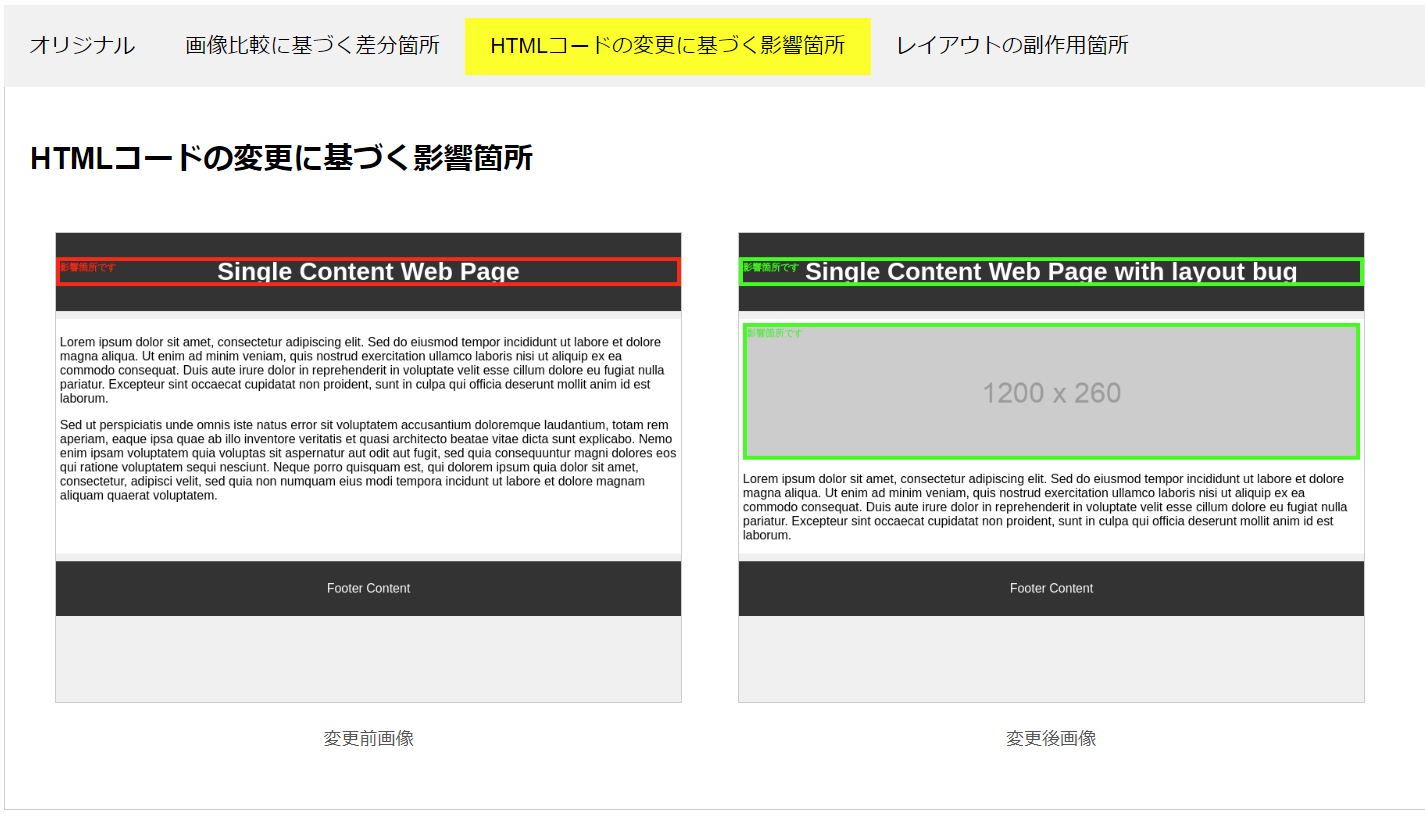
\includegraphics[width=1.0\columnwidth]{image/3_html_tab.png}
        \caption{HTMLコードの変更に基づく影響箇所表示タブを押した際の\toolName の画面例}
        \label{fig: Appearance_html_tab}
    \end{center}
\end{figure}



\section{レイアウトの副作用箇所表示タブ}\label{subsec:subeffect_tab}
レイアウトの副作用箇所表示タブを押すと、差分箇所と影響箇所に基づいて出力したレイアウトの副作用箇所を色付きの枠で強調表示した、Webページの変更前画像とWebページの変更後画像を表示する。
レイアウトの副作用箇所表示タブを押した際の画面例を、図\ref{fig: Appearance_subEffect_tab}に示す。
ここでのレイアウトの副作用箇所とは、変更前後のWebページでHTMLコードの変更による影響を受けた画面要素によって、HTMLコードを変更していない画面要素に見た目の変更があった箇所と定義する。
変更前のWebページでのレイアウトの副作用箇所は変更前画像上に赤枠で囲んで強調表示し、変更後のwebページでのレイアウトの副作用箇所は変更後画像上に緑枠で囲んで強調表示する。
このタブでは、変更前後のWebページでレイアウトの不具合を含む可能性のある箇所を目視で確認できる。
\begin{figure}[tp]
    \begin{center}
        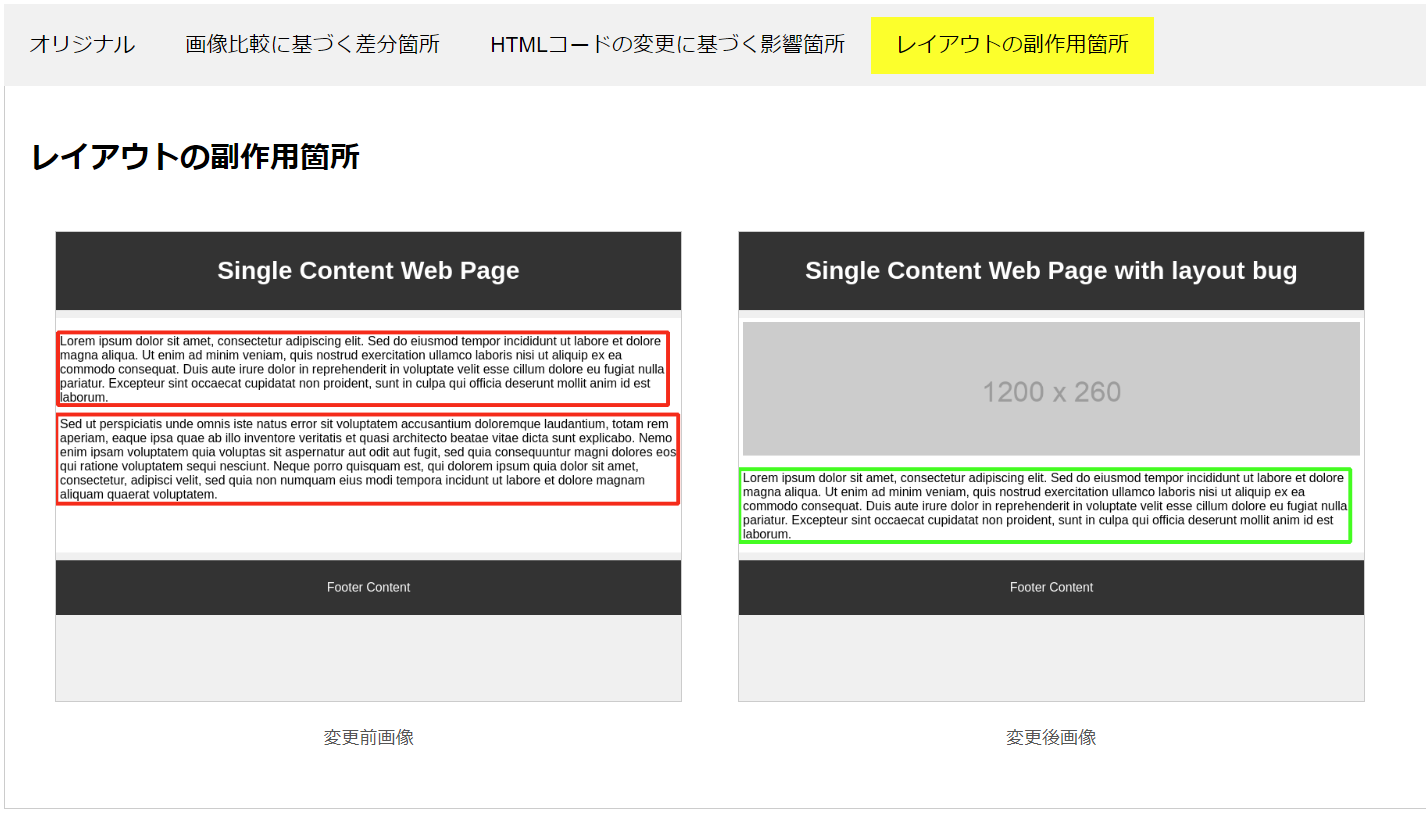
\includegraphics[width=1.0\columnwidth]{image/3_subEffect_tab.png}
        \caption{レイアウトの副作用箇所表示タブを押した際の\toolName の画面例}
        \label{fig: Appearance_subEffect_tab}
    \end{center}
\end{figure}


\chapter{MixVRTの実装}\label{cha:Implementation}
本章では、試作した\toolName の実装について説明する。
% なお、本研究で用いる、\toolName の各処理部が取得または生成する画像名を、以下に定義する。
% \begin{itemize}
%     \item Webページの変更前画像
%     \item Webページの変更後画像
%     \item 高解像度にしたWebページの変更前画像
%     \item 高解像度にしたWebページの変更後画像
%     \item 画像比較に基づく削除箇所を赤枠で囲むことで強調表示した、Webページの変更前画像
%     \item 画像比較に基づく追加箇所を緑枠で囲むことで強調表示した、Webページの変更後画像
%     \item HTMLコードにおけるbody要素内の追加とstyle要素内の追加のどちらか、
%           または両方の追加による影響を受けた箇所を赤枠で囲むことで強調表示した、Webページの変更前画像
%     \item HTMLコードにおけるbody要素内の削除とstyle要素内の削除のどちらか、
%           または両方の削除による影響を受けた箇所を緑枠で囲むことで強調表示した、Webページの変更後画像
%     \item HTMLコードの変更に基づく影響箇所を色付きの枠で囲むことで強調表示した、Webページの変更前画像
%     \item HTMLコードの変更に基づく影響箇所を色付きの枠で囲むことで強調表示した、Webページの変更後画像
%     \item レイアウトの不具合箇所を色付きの枠で囲むことで強調表示した、Webページの変更前画像
%     \item レイアウトの不具合箇所を色付きの枠で囲むことで強調表示した、Webページの変更後画像
% \end{itemize}
\par
\toolName のシステム構成を、図\ref{fig:System}に示す。
\begin{figure}[tp]
    \begin{center}
        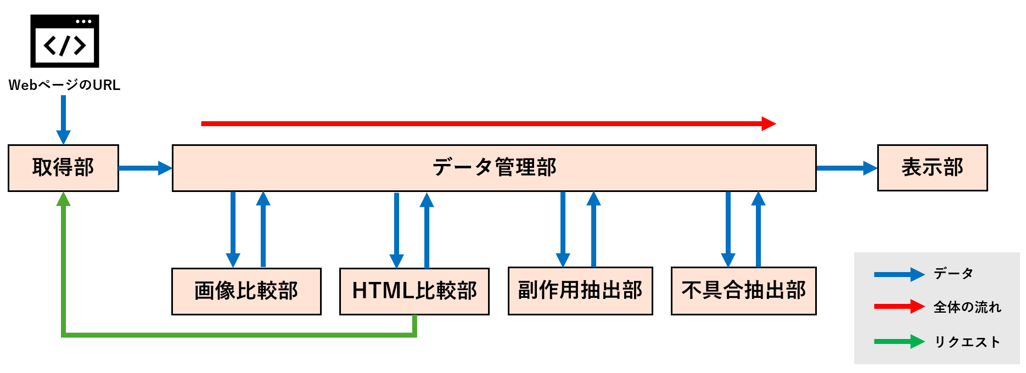
\includegraphics[width=1.0\columnwidth]{image/4_System_2.png}
        \caption{\toolName のシステム構成}
        \label{fig:System}
    \end{center}
\end{figure}
% 私の開発したツールは、まずユーザーがWebページのURLを入力します。
% このURLを受け取ると、ツールは該当するWebページから画像を取得し、
% これらの画像に対して特定の処理を行います。処理された画像は"static/images"ディレクトリに保存されます。
% そして、Flaskがローカルサーバを提供し、
% "templates"フォルダにあるHTMLコードが"static/images"ディレクトリを参照できるようになっています。
% この仕組みにより、ユーザーはローカルに立てられたFlaskサーバを通じて、
% Webページ上で生成された画像を確認することができます。
\toolName は、以下の7つの処理部から構成する。
\begin{itemize}
    \item データ管理部
    \item 取得部
    \item 画像比較部
    \item HTML比較部
    \item 副作用抽出部
    \item 不具合抽出部
    \item 表示部
          % \item 表示部
\end{itemize}
% \begin{itemize}
%     \item 取得部
%     \item 画像比較部
%           \begin{enumerate}
%               \item 差分箇所検出
%           \end{enumerate}
%     \item HTML比較部
%           \begin{enumerate}
%               \item 差分コード生成
%               \item 差分コード解析
%               \item 影響箇所強調HTMLコード生成
%           \end{enumerate}
%     \item レイアウト副作用箇所抽出部
%     \item 表示部
% \end{itemize}
以降、\toolName を構成する7つの処理部について説明する。
\par

\section{データ管理部}\label{sec:data_admin_section}
データ管理部は、システム内の各処理部間における、データの伝達を担い、他の処理部とのデータのやり取りとデータの保存を行う。
なお、本論文におけるデータとは、処理前後のWebページの画像やHTMLコードであり、
やり取りしたデータはデータ管理部が持つディレクトリに保存する。
また、取得部(\ref{sec:Web_data_get_section}節で後述)と表示部(\ref{sec:Interface_Display_Section}節で後述)のみ、データ管理部とのデータのやり取りが一方向である(図\ref{fig:System}を参照)。
% また、取得部とデータ管理部の間におけるデータのやり取りは、取得部からデータ管理部への一方向のみであり、
% データ管理部と表示部の間におけるデータのやり取りは、データ管理部から表示部への一方向のみである。
\par
データ管理部における最初のデータのやり取りは、取得部である。
取得部からデータを受け取ると、そのデータをデータ管理部のbase\_dirディレクトリに保存する。
保存した後、データがそれ以外に存在しない場合、全体の処理を終了する。
データがそれ以外に存在する場合、
画像比較部(\ref{sec:Difference_extraction_section}節で後述)、HTML比較部(\ref{sec:Affected_area_extraction}節で後述)、
副作用抽出部(\ref{sec:Layout_subEffect_extraction_section}節で後述)、不具合抽出部(\ref{sec:Layout_bug_extraction_section}節で後述)、表示部の順に
データのやり取りを行う。
データ管理部における最後のデータのやり取りは、表示部である。
表示部に出力するデータは、\ref{subsec:MixVRT_IO}節で述べた8つのPNG形式の画像のみである。
\par
各処理部との間でやり取りしたデータを保存する各ディレクトリを、以下に示す。
\begin{itemize}
    \item base\_dirディレクトリ:\\
          取得部で取得したWebページの画像とHTMLコードを保存する。
          %   \begin{itemize}
          %       \item currentディレクトリ:\\
          %             Webページの変更前画像と変更前HTMLコードを保存する。
          %       \item latestディレクトリ:\\
          %             Webページの変更後画像と変更後HTMLコードを保存する。
          %   \end{itemize}
    \item diff\_dirディレクトリ:\\
          画像比較部、HTML比較部、副作用抽出部、不具合抽出部でやり取りしたデータを保存する。
    \item disp\_dirディレクトリ:\\
          表示部に出力するデータを保存する。
          % Webページの変更前画像と変更後画像、Webページの変更前HTMLコードと変更後HTMLコードを用いて、
\end{itemize}
また、各ディレクトリに保存するデータの詳細を、以下の表に示す。
% \begin{table}[tp]
%     \caption{VariableHolder構造体が持つプロパティ}
%     \label{tb: VariableHolder}
%     \centering
%     \begin{tabular}{c|l}
%         \hline
%         プロパティ                 & \multicolumn{1}{c}{説明}   \\
%         \hline \hline
%         name                       & \begin{tabular}{l}プロパティの名前を保持する。\end{tabular}  \\ \hline
%         accessLevel                & \begin{tabular}{l}プロパティのアクセスレベルを保持する。\end{tabular}  \\ \hline
%         variableKind               & \begin{tabular}{l}型が表に示したケースのどれなのかを表す。\end{tabular}  \\ \hline
%         customAttribute            & \begin{tabular}{l}プロパティラッパの名前を保持する。\end{tabular}  \\ \hline
%         isStatic                   & \begin{tabular}{l}型プロパティの場合trueとなる。\end{tabular}  \\ \hline
%         isLazy                     & \begin{tabular}{l}遅延格納プロパティの場合trueとなる。\end{tabular}  \\ \hline
%         isConstant                 & \begin{tabular}{l}定数の場合trueとなる。\end{tabular} \\ \hline
%         literalType                & \begin{tabular}{l}型の種類がliteralの場合の型の名前を保持する。\end{tabular} \\ \hline
%         arrayType                  & \begin{tabular}{l}型の種類がarrayの場合の型の名前を保持する。\end{tabular} \\ \hline
%         dictionaryKeyType          & \begin{tabular}{l}型の種類がdictionaryの場合のキーの型の名前を保持する。\end{tabular} \\ \hline
%         dictionaryValueType        & \begin{tabular}{l}型の種類がdictionaryの場合のバリューの型の名前を保持する。\end{tabular} \\ \hline
%         tupleTypes                 & \begin{tabular}{l}型の種類がtupleの場合の型の名前を保持する。\end{tabular} \\ \hline
%         \begin{tabular}{l}conformedProtocol-\\ByOpaqueResultType\end{tabular} & \begin{tabular}{l}Opaque型が準拠するプロトコルの名前を保持する。\end{tabular} \\ \hline
%         isOptionalType             & \begin{tabular}{l}オプショナル型の場合trueとなる。\end{tabular} \\ \hline
%         initialValue               & \begin{tabular}{l}プロパティの初期値を保持する。\end{tabular} \\ \hline
%         haveWillSet                & \begin{tabular}{l}プロパティオブザーバのうちwillSetを持つ場合trueとなる。\end{tabular} \\ \hline
%         haveDidSet                 & \begin{tabular}{l}プロパティオブザーバのうちdidSetを持つ場合trueとなる。\end{tabular} \\ \hline
%         haveGetter                 & \begin{tabular}{l}getを持つ計算プロパティの場合trueとなる。\end{tabular} \\ \hline
%         haveSetter                 & \begin{tabular}{l}setを持つ計算プロパティの場合trueとなる。\end{tabular} \\ \hline
%     \end{tabular}
% \end{table}

% \toolName を2回実行した際の、データ管理部と各処理部とのやり取りを行ったデータを保存するディレクトリの構造を、以下に示す。

% % directory

% \begin{lstlisting}[language=, basicstyle=\ttfamily]
% .
% ├── base_dir/
% │   ├── (2回目実行時のタイムスタンプ)/
% │   │   ├── html/
% │   │   │   └── html_(2回目実行時のタイムスタンプ).html
% │   │   └── img/
% │   │       └── img_(2回目実行時のタイムスタンプ).png
% │   ├── current/ 
% │   │   ├── html/
% │   │   │   └── html_(1回目実行時のタイムスタンプ).html
% │   │   └── img/
% │   │       └── img_(1回目実行時のタイムスタンプ).png
% │   ├── initial/
% │   │   ├── html/
% │   │   │   └── html_(1回目実行時のタイムスタンプ).html
% │   │   └── img/
% │   │       └── img_(1回目実行時のタイムスタンプ).png
% │   └── latest/
% │       ├── html/
% │       │   └── html_(2回目実行時のタイムスタンプ).html
% │       └── img/
% │           └── img_(2回目実行時のタイムスタンプ).png
% └── diff_dir/
%      ├── diff_img_png/
%      │   ├── diff_af_img.png
%      │   └── diff_bf_img.png
%      ├── diff_rec_html_high_png/
%      │   ├── diff_rec_af_html.png
%      │   └── diff_rec_bf_html.png
%      ├── diff_rec_img_high_png/
%      │   ├── diff_rec_af_img.png
%      │   └── diff_rec_bf_img.png
%      ├── diff_html_txt/
%      │   └── diff_html.txt
%      ├── modified_html/
%      │   └── templates/
%      │       ├── modified_testPage_af.html
%      │       └── modified_testPage_bf.html
%      ├── modified_html_png/
%      │   ├── modified_testPage_af.png
%      │   └── modified_testPage_bf.png
%      ├── modifiled_html_high_png/
%      │   ├── modified_testPage_af_high.png
%      │   └── modified_testPage_bf_high.png
%      ├── original_high_png/
%      │   ├── img_af_high.png
%      │   └── img_bf_high.png
%      └── sub_effect_png/
%          ├── subEffect_af.png
%          └── subEffect_bf.png
% \end{lstlisting}

% \begin{itemize}
%     \item 取得部からデータ管理部
%     \item データ管理部から表示部
% \end{itemize}

% 5つの各処理部から受け付けるデータを、以下に示す。
% \begin{itemize}
%     \item 取得部:
%           \begin{itemize}
%               \item Webページの変更前画像と変更後画像
%           \end{itemize}
%     \item 画像比較部:
%           \begin{itemize}
%               \item 画像比較に基づく差分箇所を色付きの枠で囲むことで強調表示した、Webページの変更前画像と変更後画像
%               \item 上記の画像を高解像度にし、枠のみを抽出した、削除強調マスク画像と追加強調マスク画像
%           \end{itemize}
%     \item HTML比較部:
%           \begin{itemize}
%               \item HTMLコードの変更に基づく影響箇所を色付きの枠で囲むことで強調表示した、Webページの変更前画像と変更後画像
%               \item 上記の画像を高解像度にし、枠のみを抽出した、削除強調マスク画像と追加強調マスク画像
%           \end{itemize}
%     \item 副作用抽出部:
%           \begin{itemize}
%               \item レイアウトの副作用箇所を色付きの枠で囲むことで強調表示した、Webページの変更前画像と変更後画像
%           \end{itemize}
%     \item 不具合抽出部:
%           \begin{itemize}
%               \item レイアウトの不具合箇所を色付きの枠で囲むことで強調表示した、Webページの変更前画像と変更後画像
%           \end{itemize}
% \end{itemize}

% なお、\toolName の初回実行時は、取得部からWebページの画像とHTMLを受け取ると、\toolName 全体の処理を終了する。

\section{取得部}\label{sec:Web_data_get_section}
取得部は、テキスト端末上からWebページのURLを入力として受け取り、URLから取得したWebページの画像とHTMLコードを、データ管理部のbase\_dirディレクトリに出力する。
なお、HTML比較部から取得部に、枠付きWebページのURL(\ref{sec:Flask}節を参照)を与えて呼び出す場合があり(図\ref{fig:System}と\ref{sec:Affected_area_extraction}節を参照)、
その場合は、取得したデータをデータ管理部のdiff\_dirディレクトリに出力する。
\par
Webページの画像取得には、Selenium WebDriver(\ref{sec:Selenium_WebDriver}節を参照)を用いて、WebページのURLからWebページの画像を取得する。
なお、取得するWebページの画像は、フルページのスクリーンショット画像である。
WebページのHTMLコード取得には、Pythonライブラリの1つであるrequests(\ref{sec:requests}節を参照)を用いて、
WebページのURLからWebページのHTMLコードを取得する。

\section{画像比較部}\label{sec:Difference_extraction_section}
画像比較部は、データ管理部のbase\_dirディレクトリからWebページの変更前画像と変更後画像を受け取り、
画像比較に基づく差分箇所を色付きの枠で囲むことで強調表示した、Webページの変更前画像と変更後画像を生成する。
また、それらの画像から枠のみを残してそれ以外の部分を黒くすることで、差分箇所を囲む色付きの枠のみを抽出した、「差分箇所赤枠強調マスク画像」と「差分箇所緑枠強調マスク画像」も生成する。
生成した画像は、データ管理部のbase\_dirディレクトリに出力する。
\par
画像比較部の処理の流れを、以下に示す。
\begin{enumerate}
    \item 高解像度画像生成処理
    \item 適応的二値化処理
    \item 差分検出処理
    \item 膨張処理
    \item 輪郭検出処理
    \item 枠描画処理
\end{enumerate}
また、\toolName のテスト対象とするWebページの変更前画像と変更後画像の例を、図\ref{fig: img_original_bf_af}に示す。
\begin{figure}[tp]
    \begin{center}
        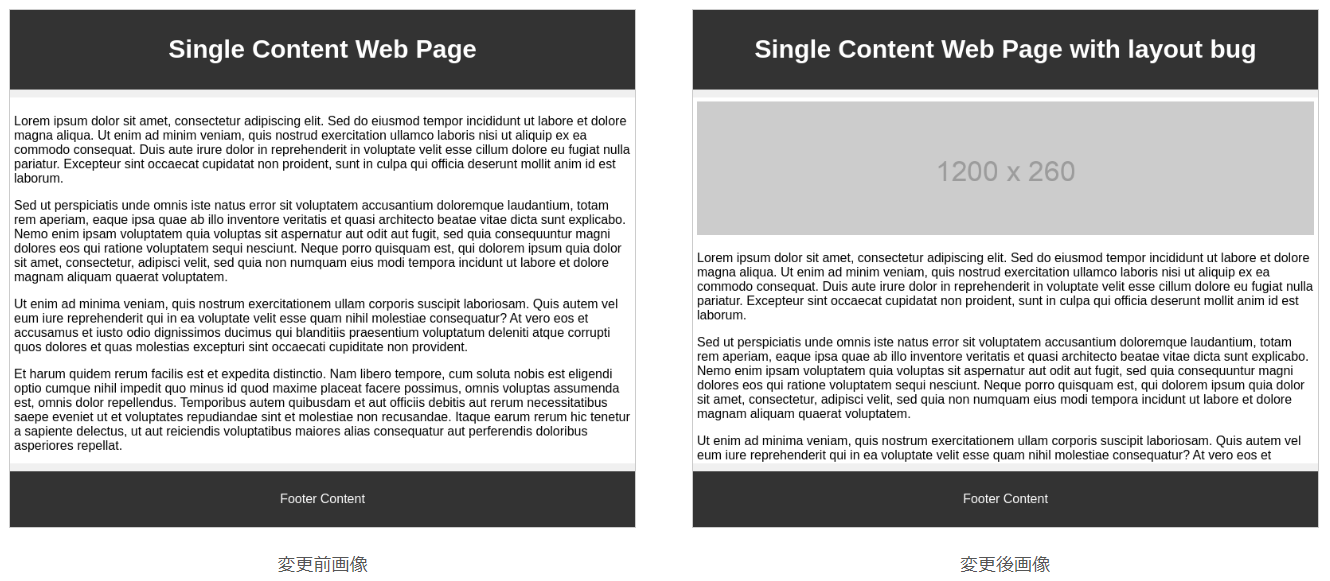
\includegraphics[width=1.0\columnwidth]{image/4_img_original_bf_af.png}
        \caption{\toolName のテスト対象とするWebページの変更前画像と変更後画像の例}
        \label{fig: img_original_bf_af}
    \end{center}
\end{figure}
以降、具体例に図\ref{fig: img_original_bf_af}を用いて、画像比較部の各処理について説明する。

\subsection{高解像度画像生成処理}\label{subsec:Generate_high_images}
高解像度画像生成処理は、図\ref{fig: img_original_bf_af}のWebページの変更前画像と変更後画像をそれぞれ高解像度画像にした、「変更前高解像度画像」と「変更後高解像度画像」を生成する。
「変更前高解像度画像」と「変更後高解像度画像」を、図\ref{fig: img_high_original_bf_af}に示す。
\begin{figure}[tp]
    \begin{center}
        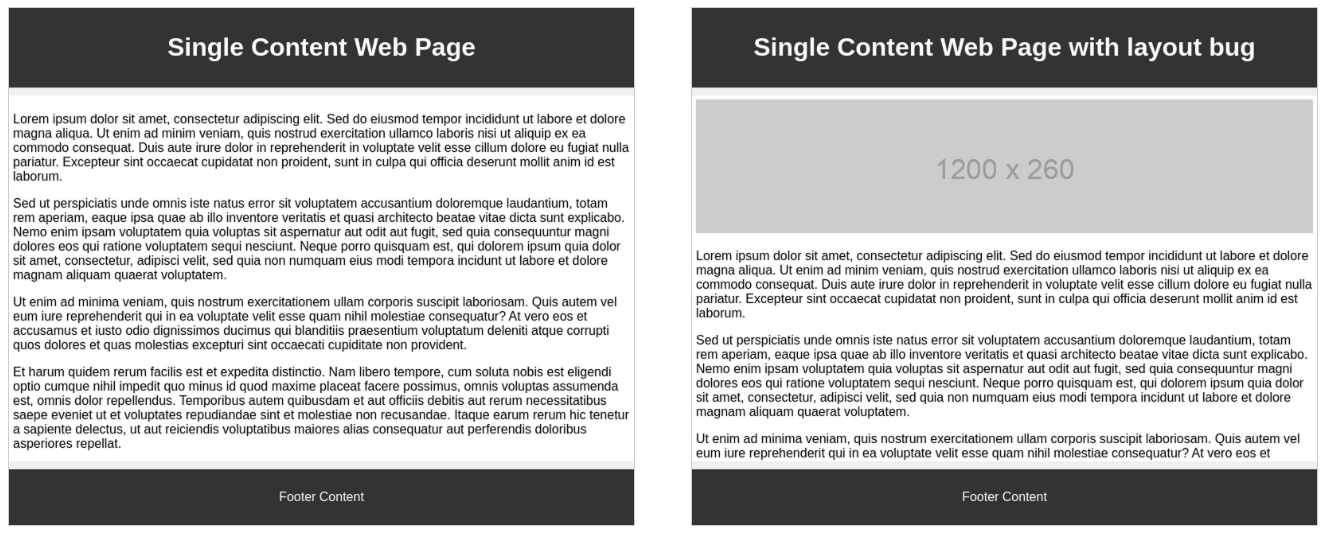
\includegraphics[width=1.0\columnwidth]{image/4_img_high_original_bf_af.png}
        \caption{「変更前高解像度画像」と「変更後高解像度画像」}
        \label{fig: img_high_original_bf_af}
    \end{center}
\end{figure}
この処理は、輪郭検出処理(\ref{subsec:contour_detection_processing}節で後述)の精度を向上するために必要である。
なお、生成した高解像度画像は他の処理部で使用するため、「変更前高解像度画像」と「変更後高解像度画像」をデータ管理部のbase\_dirディレクトリに出力する。
\par
高解像度画像を生成する流れを、以下に示す。なお、リサイズに使用するリサンプリングフィルタには、LANCZOSフィルタ(\ref{sec:pillow}節を参照)を用いる。
\begin{enumerate}
    \item PillowのImage.open関数(\ref{sec:pillow}節を参照)を用いて、Webページの画像パスから画像を読み込む。
    \item 画像の幅と高さを取得する。
    \item 画像の拡大率を設定する。本研究では、$2$とする。
    \item 画像のサイズ変更時に使用するリサンプリングフィルタを設定する。本研究では、PillowのImage.LANCZOSフィルタ(\ref{sec:pillow}節を参照)を用いる。
    \item Webページの画像を、画像の幅と高さにそれぞれ画像の拡大率を掛けたサイズの高解像度画像にリサイズする。
\end{enumerate}


\subsection{適応的二値化処理}\label{subsec:Adaptive_Binarisation}
適応的二値化処理は、図\ref{fig: img_high_original_bf_af}の「変更前高解像度画像」と「変更後高解像度画像」のそれぞれに対して、適応的二値化を行う。
この処理により、画像の一部が明るく、他の部分が暗い場合においても、全体として均一な二値化画像を生成できるため、
輪郭検出処理(\ref{subsec:contour_detection_processing}節で後述)の精度向上につながる。
処理の結果として、適応的二値化処理を行った、「変更前高解像度二値化画像」と「変更後高解像度二値化画像」を生成する。
「変更前高解像度二値化画像」と「変更後高解像度二値化画像」を、図\ref{fig: img_high_bin_bf_af}に示す。
\begin{figure}[tp]
    \begin{center}
        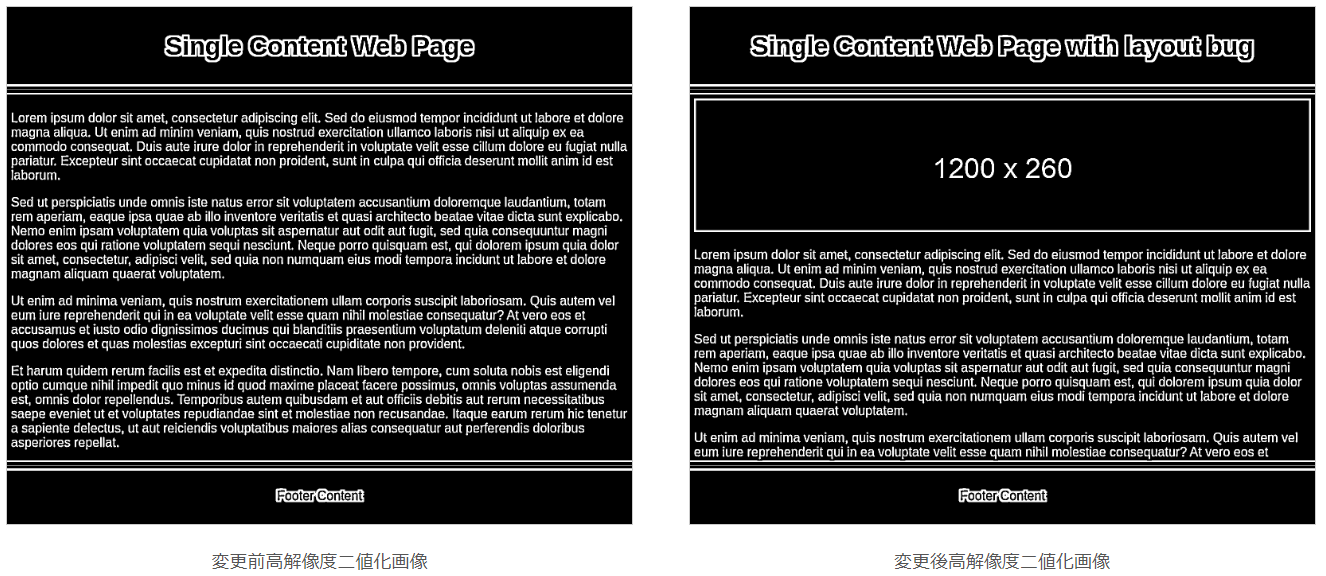
\includegraphics[width=1.0\columnwidth]{image/4_img_high_bin_bf_af.png}
        \caption{「変更前高解像度二値化画像」と「変更後高解像度二値化画像」}
        \label{fig: img_high_bin_bf_af}
    \end{center}
\end{figure}
\par
「変更前高解像度画像」と「変更後高解像度画像」に対して、それぞれ適応的二値化を行う流れを、以下に示す。
\begin{enumerate}
    \item OpenCVのimread関数(\ref{sec:opencv}節を参照)を用いて、画像を読み込む。
    \item OpenCVのcvtColor関数(\ref{sec:opencv}節を参照)を用いて、画像をグレースケール化する。
    \item OpenCVのadaptiveThreshold関数(\ref{sec:opencv}節を参照)を用いて、グレースケール画像に対して白黒反転を伴う適用的二値化を行う。
\end{enumerate}

\subsection{差分検出処理}\label{subsec:difference_detection_process}
差分検出処理は、図\ref{fig: img_high_bin_bf_af}の「変更前高解像度二値化画像」と「変更後高解像度二値化画像」に対して、差分検出を行う。
処理の結果として、Webページの変更前画像から削除された箇所と、Webページの変更後画像に追加された箇所をそれぞれ白い部分として可視化した、
「削除箇所二値化画像」と「追加箇所二値化画像」を生成する。
「削除箇所二値化画像」と「追加箇所二値化画像」を、図\ref{fig: img_del_add_bin_bf_af}に示す。
\begin{figure}[tp]
    \begin{center}
        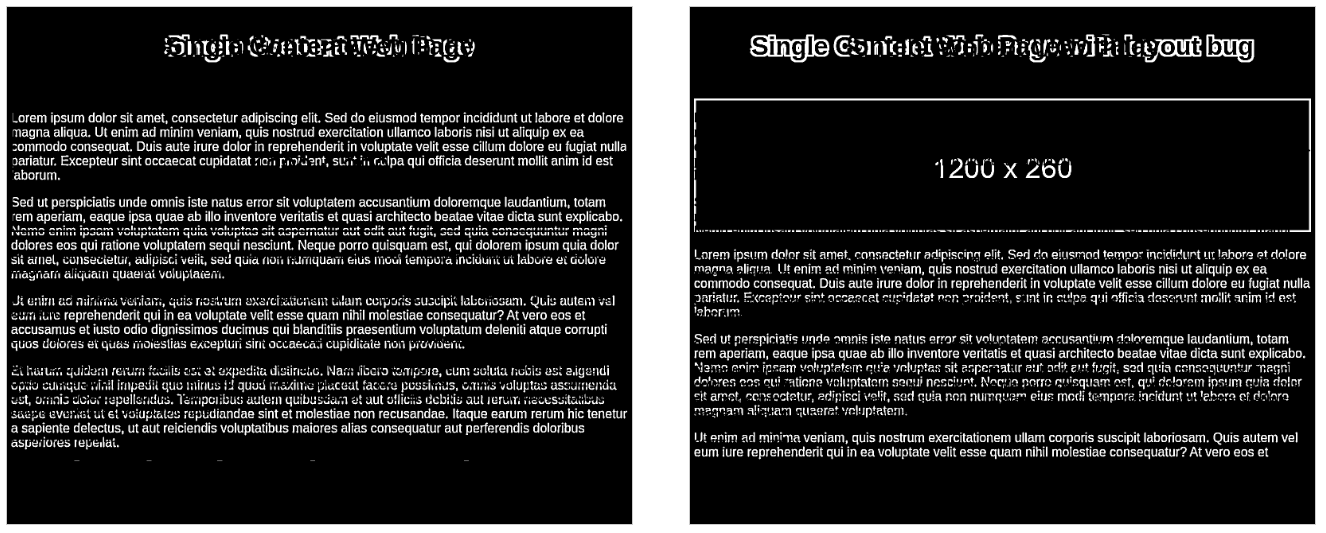
\includegraphics[width=1.0\columnwidth]{image/4_img_del_add_bin_bf_af.png}
        \caption{「削除箇所二値化画像」と「追加箇所二値化画像」}
        \label{fig: img_del_add_bin_bf_af}
    \end{center}
\end{figure}
図\ref{fig: img_del_add_bin_bf_af}を見ると、
図\ref{fig: img_high_bin_bf_af}の「変更前高解像度二値化画像」と「変更後高解像度二値化画像」を重ねたときの共通部分である白い箇所が消えており、
「変更前高解像度二値化画像」には、削除箇所が残り、「変更後高解像度二値化画像」には、追加箇所が残る。
これにより、輪郭検出処理(\ref{subsec:contour_detection_processing}節で後述)で、削除箇所を赤枠で、追加箇所を緑枠で囲むことができる。
\par
「変更前高解像度二値化画像」と「変更後高解像度二値化画像」に対して、差分検出処理を行う流れを、以下に示す。
\begin{enumerate}
    \item OpenCVのsubtract関数(\ref{sec:opencv}節を参照)の第一引数に「変更前高解像度二値化画像」を指定し、
          第二引数に「変更後高解像度二値化画像」を指定する。
    \item 1のsubtract関数によって、変更前の画像には存在するが変更後の画像には存在しない箇所を可視化した「削除箇所二値化画像」を生成する。
    \item subtract関数(\ref{sec:opencv}節を参照)の第一引数に「変更後高解像度二値化画像」を指定し、
          第二引数に「変更前高解像度二値化画像」を指定する。
    \item 3のsubtract関数によって、変更後の画像には存在するが変更前の画像には存在しない箇所を可視化した「追加箇所二値化画像」を生成する。
\end{enumerate}

\subsection{膨張処理}\label{subsec:dilation}
% (\ref{sec:dilation}節を参照)
膨張処理は、「削除箇所二値化画像」と「追加箇所二値化画像」のそれぞれの白い部分の形状とサイズを強調する。
この処理により、削除箇所と追加箇所の輪郭検出処理(\ref{subsec:contour_detection_processing}節で後述)を高める。
処理の結果として、膨張処理を行った、「削除箇所強調二値化画像」と「追加箇所強調二値化画像」を生成する。
「削除箇所強調二値化画像」と「追加箇所強調二値化画像」を、図\ref{fig: img_del_add_highlight_bin}に示す。
\begin{figure}[tp]
    \begin{center}
        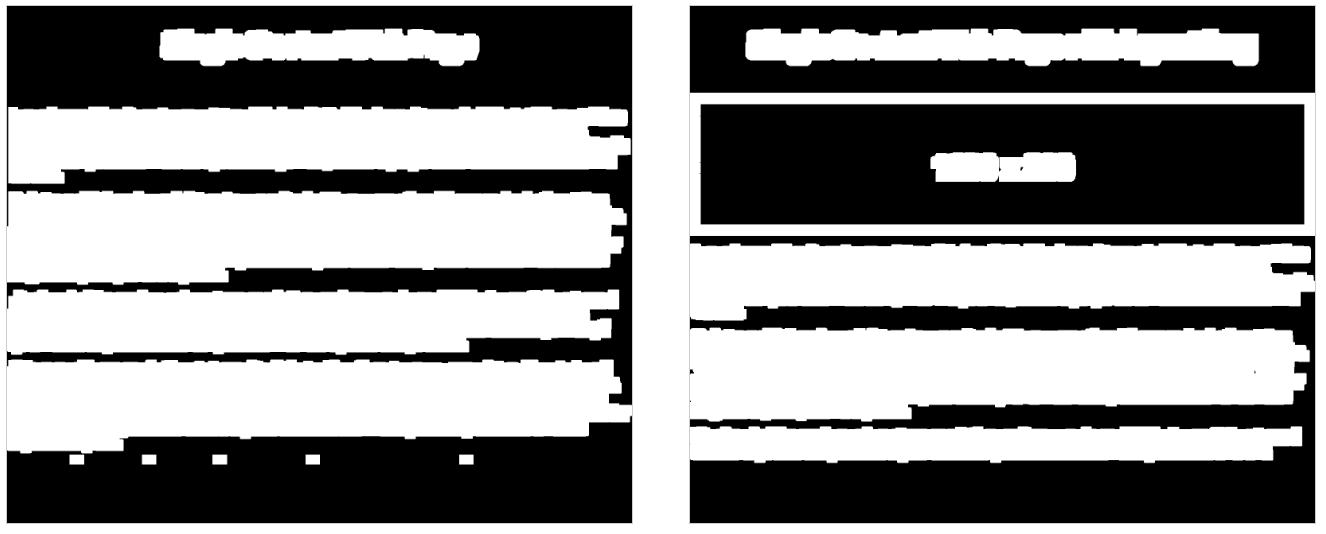
\includegraphics[width=1.0\columnwidth]{image/4_img_del_add_highlight_bin.png}
        \caption{「削除箇所強調二値化画像」と「追加箇所強調二値化画像」}
        \label{fig: img_del_add_highlight_bin}
    \end{center}
\end{figure}
\par
「削除箇所二値化画像」と「追加箇所二値化画像」に対して、膨張処理を適用する流れを、以下に示す。
\begin{enumerate}
    \item 特定の形状とサイズを持つカーネルを設定する。本研究では、5x5ピクセルの正方形カーネルを採用する。
    \item 設定したカーネルを用いて、膨張処理を適用する。適用後、画像内の削除箇所または追加箇所が拡大する。
    \item 2の膨張処理を複数回適用する。本研究では、膨張処理を6回繰り返すことで削除箇所または追加箇所を強調する。
    \item 膨張処理によって生成した「削除箇所強調二値化画像」と「追加箇所強調二値化画像」を輪郭検出処理に渡す。
\end{enumerate}

\subsection{輪郭検出処理}\label{subsec:contour_detection_processing}
輪郭検出処理は、OpenCVのfindContours関数(\ref{sec:opencv}節を参照)を用いて、図\ref{fig: img_del_add_highlight_bin}の「削除箇所強調二値化画像」と「追加箇所強調二値化画像」に対して、
削除箇所の輪郭と追加箇所の輪郭をそれぞれ検出する。
この処理の結果として、削除箇所の輪郭リストと追加箇所の輪郭リストを取得する。

\subsection{枠描画処理}\label{subsec:Bounding box drawing process}
枠描画処理は、Webページの変更前画像と変更後画像に対して、
輪郭検出処理(\ref{subsec:contour_detection_processing}節を参照)で取得した輪郭リストを用いて、
図\ref{fig: img_diff_highlight}に示した、
画像比較に基づく差分箇所を、色付きの枠で囲むことで強調表示した、Webページの変更前画像と変更後画像を生成する。
\begin{figure}[tp]
    \begin{center}
        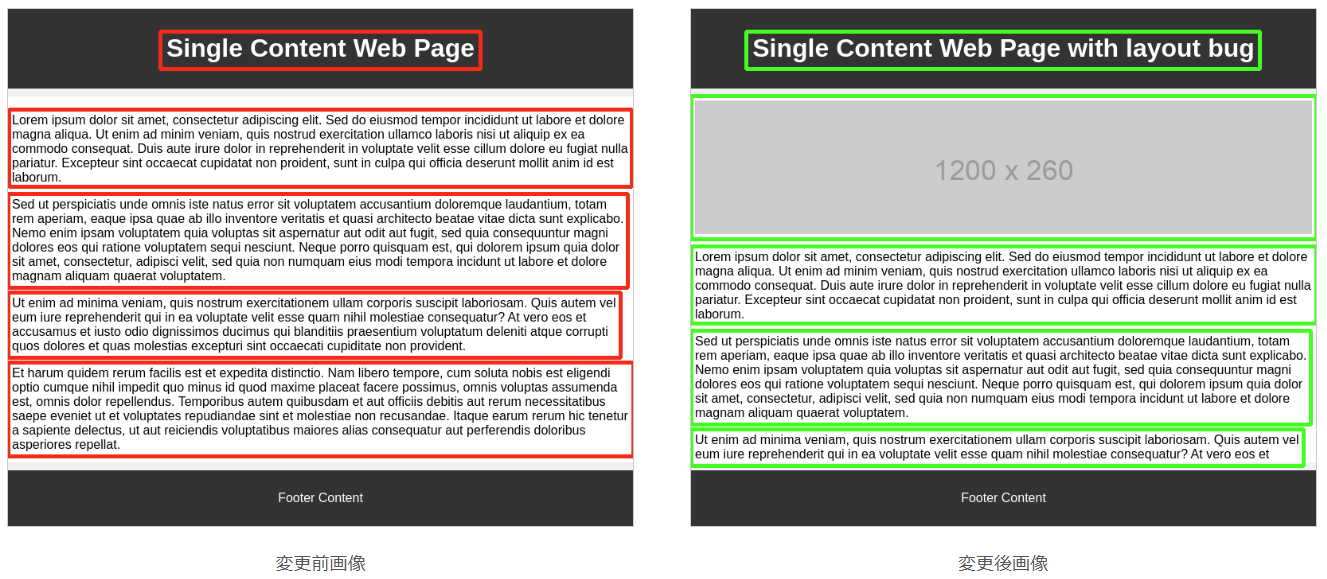
\includegraphics[width=1.0\columnwidth]{image/4_img_diff_highlight.png}
        \caption{画像比較に基づく差分箇所を、色付きの枠で囲むことで強調表示した、Webページの変更前画像と変更後画像}
        \label{fig: img_diff_highlight}
    \end{center}
\end{figure}
また、それらの画像から枠のみを残してそれ以外の部分を黒くすることで、差分箇所を囲む色付きの枠のみを抽出した、
「差分箇所赤枠強調マスク画像」と「差分箇所緑枠強調マスク画像」を生成する。
「差分箇所赤枠強調マスク画像」と「差分箇所緑枠強調マスク画像」を、図\ref{fig: img_diff_highlight_mask}に示す。
\begin{figure}[tp]
    \begin{center}
        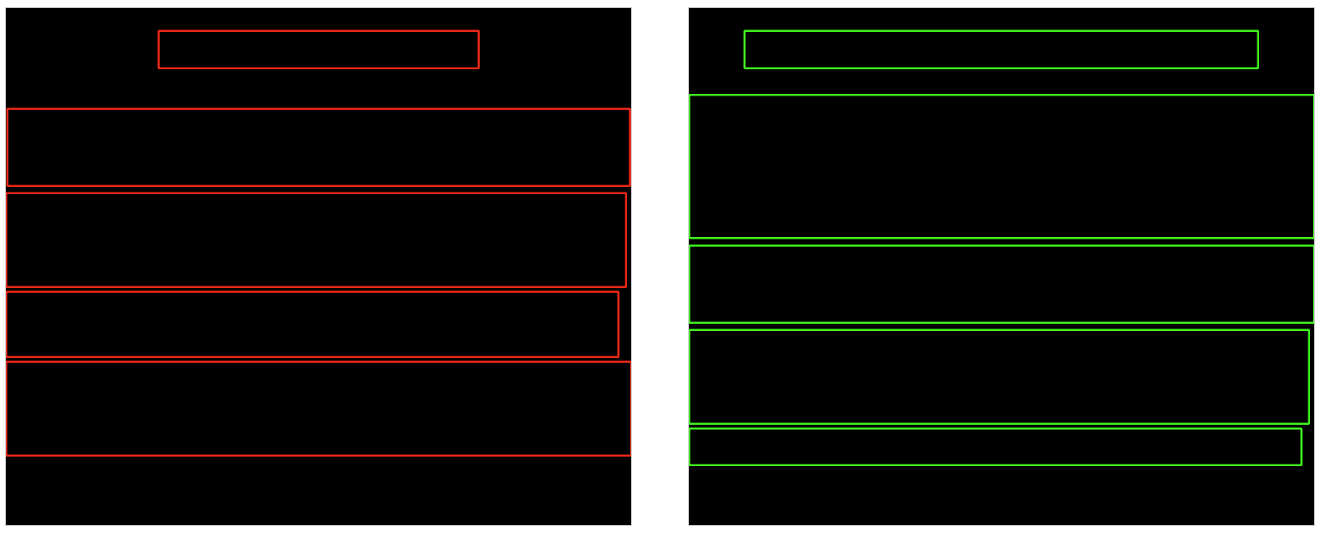
\includegraphics[width=1.0\columnwidth]{image/4_img_diff_highlight_mask.png}
        \caption{「差分箇所赤枠強調マスク画像」と「差分箇所緑枠強調マスク画像」}
        \label{fig: img_diff_highlight_mask}
    \end{center}
\end{figure}
\par
枠描画処理の流れを、以下に示す。
\begin{enumerate}
    \item cv2.boundingRect関数(\ref{sec:opencv}節を参照)を用いて、輪郭リストの各要素である輪郭データから、輪郭を囲む矩形の座標と幅、高さを取得する。
    \item 取得した矩形情報を引数に指定したcv2.rectangle関数(\ref{sec:opencv}節を参照)を用いて、Webページの変更前画像上に赤枠、Webページの変更後画像上に緑枠を描画する。
    \item np.zeros関数(\ref{sec:numpy}節を参照)を用いて、Webページの変更前画像と変更後画像のそれぞれと同じサイズの黒画像を生成する。
    \item 取得した矩形情報を引数に指定したcv2.rectangle関数を用いて、生成した2つの黒画像に対して、一方の黒画像には赤枠を、もう一方の黒画像には緑枠を描画する。
\end{enumerate}


%%%% HTML比較 %%%%
% 画像比較部は、データ管理部のbase\_dirディレクトリからWebページの変更前画像と変更後画像を受け取り、
% 画像比較に基づく差分箇所を色付きの枠で囲むことで強調表示したWebページの変更前画像と変更後画像を生成する。
% また、それらの画像から枠のみを残してそれ以外の部分を黒くすることで、差分箇所を囲む色付きの枠のみを抽出した、「差分箇所赤枠強調マスク画像」と「差分箇所緑枠強調マスク画像」も生成する。
% 生成した画像は、データ管理部のbase\_dirディレクトリに出力する。
% \par
% 画像比較部の処理の流れを、以下に示す。
% \begin{enumerate}
%     \item 高解像度画像生成処理
%     \item 適応的二値化処理
%     \item 差分検出処理
%     \item 膨張処理
%     \item 輪郭検出処理
%     \item 枠描画処理
% \end{enumerate}
% また、\toolName のテスト対象とするWebページの変更前画像と変更後画像の例を、図\ref{fig: img_original_bf_af}に示す。
% \begin{figure}[tp]
%     \begin{center}
%         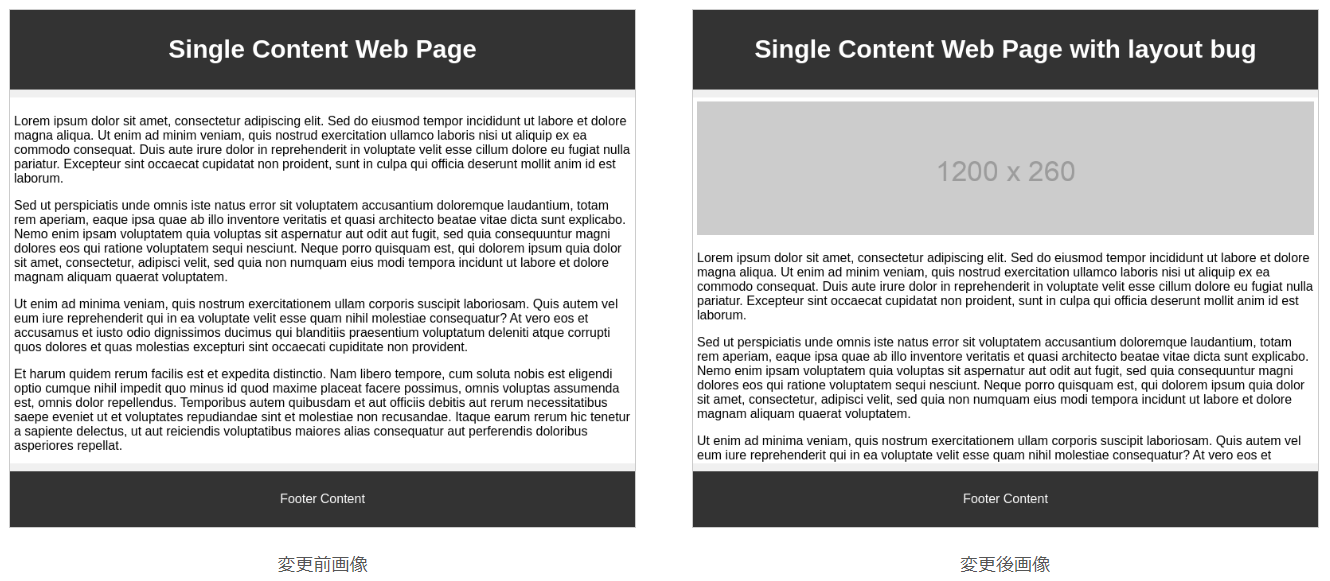
\includegraphics[width=1.0\columnwidth]{image/4_img_original_bf_af.png}
%         \caption{\toolName のテスト対象とするWebページの変更前画像と変更後画像の例}
%         \label{fig: img_original_bf_af}
%     \end{center}
% \end{figure}
% 以降、具体例に図\ref{fig: img_original_bf_af}を用いて、画像比較部の各処理について説明する。
\section{HTML比較部}\label{sec:Affected_area_extraction}
HTML比較部は、データ管理部のbase\_dirディレクトリからWebページの変更前HTMLコードと変更後HTMLコードを受け取り、
HTMLコードの変更に基づく影響箇所を色付きの枠で囲むことで強調表示した、Webページの変更前画像と変更後画像を生成する。
また、それらの画像から枠のみを残してそれ以外の部分を黒くすることで、影響箇所を囲む色付きの枠のみを抽出した、「影響箇所赤枠強調マスク画像」と「影響箇所緑枠強調マスク画像」も生成する。
生成した画像は、データ管理部のbase\_dirディレクトリに出力する。
\par
HTML比較部の処理の流れを、以下に示す。
\begin{enumerate}
    \item 差分コード生成処理
    \item 差分コード解析処理
    \item 影響箇所強調HTMLコード生成処理
    \item 枠抽出処理
\end{enumerate}
以降、図\ref{fig: img_original_bf_af}の例で挙げたWebページの、変更前HTMLコードと変更後HTMLコードを具体例に、
HTML比較部の各処理について説明する。

\subsection{差分コード生成処理}\label{subsec:diff_file_generate}
差分コード生成処理は、Webページの変更前HTMLコードと変更後HTMLコードを行ごとに比較して、txt形式の差分コードを生成する。
生成したtxt形式の差分コードの例を、ソースコード\ref{lst:diff_html}に示す。
ソースコード\ref{lst:diff_html}の3行目を見ると、先頭に"-"が付いており、この行は削除行であることを示す。
また、ソースコード\ref{lst:diff_html}の4行目および8行目を見ると、先頭に"+"が付いており、この行は追加行であることを示す。
このように、生成したtxt形式の差分コードには、コードの追加行の先頭に"+"、削除行の先頭に"-"を付加する。
\begin{figure}[tp]
    \begin{lstlisting}[language=HTML, caption=生成したtxt形式の差分コードの例, label=lst:diff_html]
<body>
    <header>
-         <h1>Single Content Web Page</h1>
+         <h1>Single Content Web Page with layout bug</h1>
    </header>
    <div class="container">
        <div class="main-content">
+             <img src="https://via.placeholder.com/1200x260" alt="Placeholder Image">
              // テキスト文省略
        </div>
    </div>
    <footer>
        <p>Footer Content</p>
    </footer>
</body>
    \end{lstlisting}
\end{figure}
\par
差分コードを生成する処理を、以下に示す。
\begin{enumerate}
    \item 変更前HTMLコードと変更後HTMLコードをそれぞれHTMLデータとして読み込む。
    \item HTMLデータ内の$<$p$>$タグ内のテキスト内に存在する余分な空白や改行を取り除く(\ref{sec:text_change}節を参照)ために、以下を行う。
          \begin{enumerate}
              \item 変更前と変更後のHTMLデータを解析するためのBeautifulSoupオブジェクト(\ref{sec:beautifulsoup}節を参照)をそれぞれ初期化する。
              \item BeautifulSoupオブジェクトに対して、find\_all関数(\ref{sec:beautifulsoup}節を参照)を用い、HTMLデータ内の全ての$<$p$>$タグを格納したリストを生成する。
              \item get\_text関数(\ref{sec:beautifulsoup}節を参照)を用いて、生成したリストの各要素内における$<$p$>$タグのテキストを取得する。
              \item Pythonの文字列関数であるsplit関数を用いて、取得した各テキストを空白文字で分割する。
              \item Pythonの文字列関数であるjoin関数を用いて、分割したテキストを再び空白文字で連結する。
              \item BeautifulSoupオブジェクトをstring型に変換し、HTMLデータ形式に戻す。
          \end{enumerate}
    \item difflib(\ref{sec:difflib}節を参照)のDifferクラスとcompare関数を用いて、2つのHTMLデータ間を行ごとに比較し、差分コードを生成する。
    \item 生成した差分コードから、行の先頭が"?"から始まる行を除外する。
    \item 差分コードをtxt形式で保存する。
\end{enumerate}

% \subsection{差分コード解析処理}\label{subsec:diff_file_analyze}
% 差分コード解析処理は、差分コード生成処理から差分コードを受け取り、差分コードからbody要素内の変更箇所とstyle要素内の変更箇所を検出する。
% \par
% 差分コードを解析する処理を、以下に示す。

% 枠付きHTMLコード生成するためには、以下の処理を行う。
% body要素内の変更箇所を検出する。
% 差分コードの先頭の行に対して、以下の処理を行う。
% 1.body要素外であるか判定する。body要素外ならば、以下の処理を行う。
% 1. 先頭行が"-"であれば、
% body要素内の各先頭行に"+"または"-"がある箇所を探す。
% "+"や"-"であれば、その行に対して以下の操作を行う。
% 1."+"または"-"を削除する。
% 2.行にimgタグが含まれている場合、img用の枠を囲むCSSクラスを追加する。
% 3.行にimgタグが含まれていない場合、行中に開始タグが存在するかを確認する。
% 4.行中に開始タグが存在する場合は、タグ内にclass属性が既にあるかどうか確認する。行中に開始タグが存在しない場合は、何もしない。
% 5.class属性があれば、class=""の中の末尾に枠をつけるクラスを追加する。
% 6.class属性が無ければ、終了タグ直前に枠をつけるクラスを追加する。

% body要素内の変更箇所に枠をつけるCSSクラスを追加する。
% style要素内の変更箇所を検出する。
% style要素内の変更箇所に枠をつけるCSSクラスを追加する。

\subsection{枠付きHTMLコード生成処理}\label{subsec:modified_html_generate}
【TODO: 処理を整理する必要あり】\\
枠付きHTMLコード生成処理は、差分コード生成処理から差分コードを受け取り、枠付き変更前HTMLコードと枠付き変更後HTMLコードを生成する。
なお、枠付き変更前HTMLコードは、影響箇所(\ref{cha:Function}を参照)における削除箇所に赤枠をつけるCSSクラスを付与した、変更前HTMLコードと定義する。
また、枠付き変更後HTMLコードは、影響箇所における追加箇所に緑枠をつけるCSSクラスを付与した、変更後HTMLコードと定義する。
\par
差分コードから、枠付き変更前HTMLコードと枠付き変更後HTMLコードを生成する処理を、以下に示す。
\begin{enumerate}
    \item CSSセレクタ抽出処理
    \item body要素解析処理
    \item CSSクラス定義処理
\end{enumerate}

\subsubsection{CSSセレクタ抽出処理}\label{subsubsec: style_analysis}
CSSセレクタ抽出処理は、style要素内において変更があったCSSセレクタ\cite{CssSelector}を、差分コードから全て抽出する。
抽出したCSSセレクタは、リストにそれぞれ格納し、CSSクラス定義処理(\ref{subsubsec: css_define}節に後述)に出力する。
sytle要素解析処理の流れを、以下に示す。
\begin{enumerate}
    \item 変更があったCSSセレクタを格納するリストであるchanged\_selectorsを、空リストとして初期化する。
    \item 現在処理中のCSSセレクタを保持するための変数であるcurrent\_selectorの値を、Noneに初期化する。
    \item 差分コードの全ての行に対して、先頭行から順に1行ずつ文字列の判定をし、判定結果に応じて、以下の処理を行う。
          \begin{enumerate}
              \item CSSセレクタの開始を示す"\{"を含む行を見つけた場合:
                    \begin{enumerate}
                        \item 行中のCSSセレクタのみを抽出する。
                        \item changed\_selectors内に抽出したセレクタが存在せず、かつ、行が変更を示す"+"、または、"-"で始まる場合、
                              CSSセレクタをchanged\_selectorsに格納する。
                        \item current\_selectorの値にCSSセレクタを格納し、現在処理中のCSSセレクタを更新する。
                    \end{enumerate}
              \item CSSセレクタの終了を示す"\}"を含む行を見つけた場合:
                    \begin{enumerate}
                        \item current\_selectorの値にNoneを格納し、現在処理中のCSSセレクタをリセットする。
                        \item 3に戻る。
                    \end{enumerate}
              \item current\_selectorの値にCSSセレクタが格納されており、行が変更を示す"+"、または、"-"で始まる場合:
                    \begin{enumerate}
                        \item changed\_selectors内に、current\_selectorに格納されているCSSセレクタが存在しないならば、
                              そのCSSセレクタをchanged\_selectorsに格納する。
                    \end{enumerate}
          \end{enumerate}
    \item changed\_selectorsをCSSクラス定義処理に出力する。
\end{enumerate}

\subsubsection{body要素解析処理}\label{subsubsec: body_analysis}
body要素解析処理は、変更前後のWebページでbody要素内に変更があったタグ要素のstyle属性にCSSクラスを付与しつつ、
枠付き変更前HTMLコードと枠付き変更後HTMLコードを生成する中間の処理を行う。
body要素解析処理の流れを、以下に示す。
なお、枠付き変更前HTMLコードの各行を格納するリストmodified\_before\_linesと枠付き変更後HTMLコードの各行を格納するリストmodified\_after\_linesを空リストとして初期化する。
また、処理を行う行が削除行であると判定する変数flag\_beforeと追加行であると判定する変数flag\_afterをそれぞれFalseで初期化する。
さらに、差分コードの先頭行から順に各行に対して、以下の処理を行うものとする。
\begin{enumerate}
    \item 行がbody要素外の場合:
          \begin{enumerate}
              \item 行の先頭が"-"の場合、modified\_before\_linesに行を追加する。
              \item 行の先頭が"+"の場合、modified\_after\_linesに行を追加する。
              \item 行の先頭がそれ以外の場合、modified\_before\_linesとmodified\_after\_linesの両方に行を追加する。
          \end{enumerate}
    \item 行がbody要素内の場合:
          \begin{enumerate}
              \item (b)と(c)はif-elseブロック
              \item 行の先頭が"-"または"+"の場合:
                    \begin{enumerate}
                        \item 行の先頭が"-"の場合、flag\_beforeの値をTrueにし、"-"を取り除く
                        \item 行の先頭が"+"の場合、flag\_afterの値をTrueにし、"+"を取り除く
                        \item 行中に"\textless img"を含む場合:
                              \begin{enumerate}
                                  \item imgタグ用のCSSクラスを付与したdivタグでimgタグを囲む。
                              \end{enumerate}
                        \item 行中に"\textless img"を含まない場合:
                              \begin{enumerate}
                                  \item 行中に"class="を含む場合、開始タグのstyle属性にbody要素用のCSSクラスを付与する。
                                  \item 行中に"class="を含まない場合、開始タグの終了記号直前にbody要素用のCSSクラスを付与する。
                              \end{enumerate}
                    \end{enumerate}
              \item 行の先頭がそれ以外の場合:\\
                    flag\_beforeとflag\_afterの両方の値をFalseにする。
              \item (e)と(f)と(g)はif-elif-elseブロック
              \item flag\_beforeの値がTrue、 かつ、flag\_afterの値がFalseの場合、modified\_before\_linesに行を追加する。
              \item flag\_beforeの値がFalse、 かつ、flag\_afterの値がTrueの場合、modified\_after\_linesに行を追加する。
              \item それ以外の場合、modified\_before\_linesとmodified\_after\_linesの両方に行を追加する。
          \end{enumerate}
\end{enumerate}

\subsubsection{CSSクラス定義処理}\label{subsubsec: css_define}
CSSクラス定義処理は、body要素解析処理から未完成の枠付き変更前HTMLコードと枠付き変更後HTMLコードのそれぞれに対して、
style要素内の末尾にCSSクラスの定義を追記する。
【TODO: 処理内容を書く】

\subsection{枠抽出処理}\label{subsec:frame_extraction}
枠抽出処理は、Webページの変更前画像と枠付きを行ったWebページの変更前画像を比較し、赤枠のみを抽出した画像を生成する。
また、Webページの変更後画像と枠付きを行ったWebページの変更後画像を比較し、緑枠のみを抽出した画像を生成する。
生成した画像は、レイアウトの副作用抽出部に出力する。
\par
枠抽出処理の流れを、以下に示す。
\begin{enumerate}
    \item 枠付きHTMLコードをローカルサーバ上(\ref{sec:Flask}節を参照)でWebページとして公開する
    \item 取得部を用いて、枠付きHTMLコードをもとにしたWebページの画像を取得する
    \item Webページの変更前画像と枠付きを行ったWebページの変更前画像を比較し、赤枠のみを抽出した変更前画像を生成する
    \item Webページの変更後画像と枠付きを行ったWebページの変更後画像を比較し、緑枠のみを抽出した変更後画像を生成する
\end{enumerate}

% \section{影響箇所検出部}\label{sec:Affected_area_extraction}
% HTMLコードの変更に基づく影響箇所抽出部は、Webページ情報取得部で取得した変更前後のWebページのHTMLコードを用いて影響箇所を特定する。
% 概要としては、差分コードを生成し、差分コードから枠付き処理を行った変更前後のHTMLコードを生成した後、そのHTMLコードをFlaskのテンプレートエンジンを用いてWebページを表示し、Webページ情報取得部によってそのWebページの画像を取得する。
% 元のWebページ画像と枠付き処理をしたWebページ画像を比較して枠のみを抽出する。
% 具体的には、まず、Pythonライブラリの一つであるdifflibモジュールを用いて、変更前後のHTMLコードから差分コードを生成する。
% 生成した差分コードは、コードの追加行には"+", 削除行には"-", 変更前後のHTMLコードにどちらにも存在しない行には"?"が先頭に付き、"?"を除いた差分コードを解析対象とする。
% 差分コードは、bodyタグ内とstyleタグ内を対象とする。
% もし、bodyタグ内で先頭に"+"や"-"があれば、コードの追加や削除、変更があったとして、その箇所に枠付き処理を行うCSSクラスを追加し、先頭の"+"か"-"を削除する。
% styleタグ内の場合は、CSSクラスのセレクタ名のみの変更やスタイルのみの変更、またはその両方の変更があったCSSクラスを対象として、そのCSSクラスに対して枠付きを行うスタイルを適用する。
% この場合においても、解析した行の先頭に"+", "-"があれば削除する。
% 差分コードから枠付き処理を行った変更前後のHTMLコードを生成した後は、そのHTMLコードをFlaskのテンプレートエンジンを用いてWebページとして表示し、そのWebページの画像を取得する。
% そして、元のWebページ画像と枠付き処理をしたWebページ画像を比較して枠のみを抽出する。
\section{副作用抽出部}\label{sec:Layout_subEffect_extraction_section}
副作用抽出部は、データ管理部のdiff\_dirディレクトリから「差分箇所赤枠強調マスク画像」と「差分箇所緑枠強調マスク画像」、「影響箇所赤枠強調マスク画像」と「影響箇所緑枠強調マスク画像」を受け取り、
これらの画像から、レイアウトの副作用箇所を抽出した、変更前画像と変更後画像を生成する。
生成した画像は、データ管理部のdiff\_dirディレクトリに出力する。
副作用抽出部の処理の流れを、以下に示す。
\begin{enumerate}
    \item 「差分箇所赤枠強調マスク画像」と「影響箇所赤枠強調マスク画像」をcv2.imread関数で読み込む。
    \item cvtColor関数でグレースケール化する。
    \item threshold関数で二値化を行う。
    \item 二値化した「差分箇所赤枠強調マスク画像」に対して、cv2.findContours関数で輪郭リストcontours\_img\_bfを取得する。
    \item 二値化した「影響箇所赤枠強調マスク画像」に対して、cv2.findContours関数で輪郭リストcontours\_html\_bfを取得する。
    \item contours\_img\_bfの各輪郭要素の数だけループして、以下の処理を行う。
          \begin{enumerate}
              \item contours\_html\_bfの各輪郭要素の数だけループして、以下の処理を行う。
                    \begin{enumerate}
                        \item  contours\_img\_bfとcontours\_html\_bfのそれぞれの輪郭要素のバウンディングボックスを取得する。
                        \item バウンディングボックスが重なっているか判定する
                              \begin{enumerate}
                                  \item  重なっている場合は、重なり部分のバウンディングボックスの面積を計算する。
                                        小さい方のバウンディングボックスの面積を計算する。
                                        重なり部分のバウンディングボックスの面積が、小さい方のバウンディングボックスの面積の6割を超えれば、
                                        大きい方のバウンディングボックスと小さい方のバウンディングボックスが重なっていると判定し、Trueを返す。そうでなければ、Falseを返す。
                                  \item 重なっていない場合は、Falseを返す。
                              \end{enumerate}
                    \end{enumerate}
              \item matchの値がTrueなら、ループ処理から抜ける。
          \end{enumerate}
    \item matchの値がTrueなら、contours\_img\_bfの輪郭要素をunique\_contours\_bfに格納する。
    \item 「差分箇所緑枠強調マスク画像」上の各緑枠と「影響箇所赤枠強調マスク画像」上の各緑枠を比較する。
\end{enumerate}
% レイアウトの副作用抽出部は、画像比較に基づく差分箇所とHTMLコードの変更に基づく影響箇所を用いて、レイアウトの副作用箇所を抽出する。
% 具体的には、差分箇所を囲む枠と影響箇所を囲む枠同士を比較する。比較の仕方は、枠の重なり度合を判定する。
% まず、枠が重なっているかどうかを判定する。次に、枠が重なっている場合に、重なり部分が小さい方の枠の面積の6割以上であれば枠が一致すると判定する。
% 最終的に、一致しない枠のみを抽出し、一致しない赤枠をWebページの変更前画像に、一致しない緑枠をWebページの変更後画像に描画し、保存する。
% 「」と「」を、図\ref{fig: subeffect_name}に示す。
\begin{figure}[tp]
    \begin{center}
        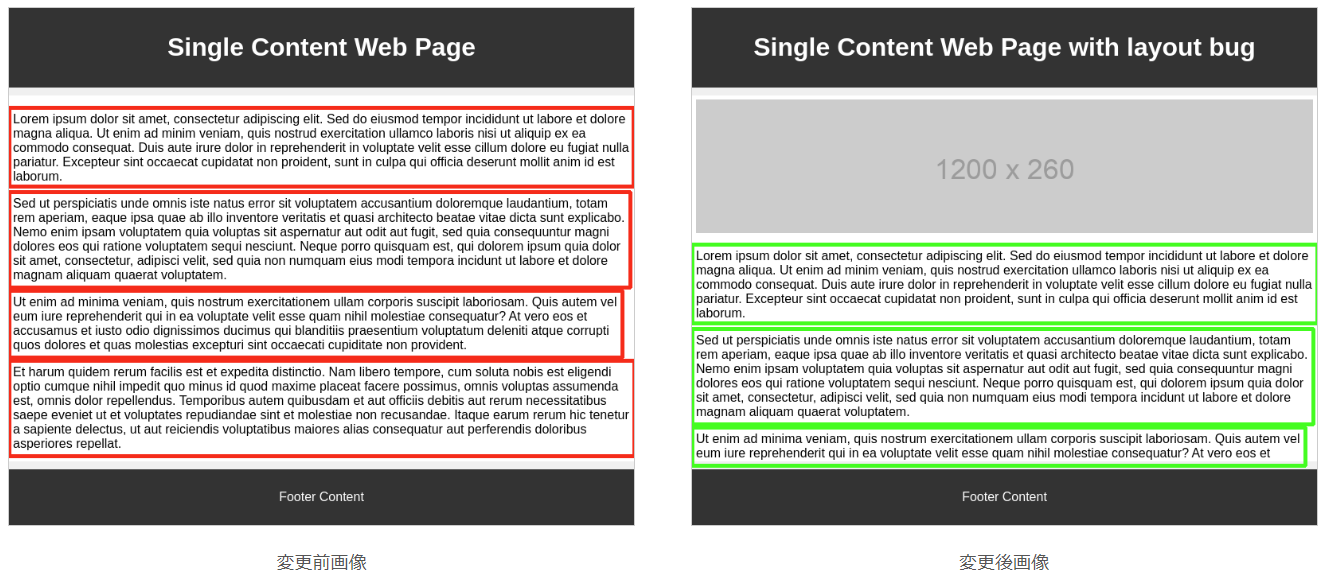
\includegraphics[width=1.0\columnwidth]{image/4_subeffect_name.png}
        \caption{レイアウト副作用箇所を色付きの枠で囲むことで強調表示した、変更前画像と変更後画像}
        \label{fig: subeffect_name}
    \end{center}
\end{figure}
\par

\section{不具合抽出部}\label{sec:Layout_bug_extraction_section}
レイアウト不具合抽出部は、データ管理部のdiff\_dirディレクトリから~画像を受け取り、
副作用抽出部から抽出したレイアウトの副作用箇所から、レイアウトの不具合箇所を抽出する。
具体的には、\ref{sec:Layout_subEffect_extraction_section}節で抽出したレイアウトの副作用箇所を囲んだ各赤枠内の領域と、レイアウトの副作用箇所を囲んだ各緑枠内の領域を比較する。
その後、赤枠内の領域と緑枠内の領域をabsdiff関数(\ref{sec:opencv}節を参照)で絶対差分を計算して類似度を求める。
類似度が9割を超えれば、レイアウトの不具合は無いと判定し、比較した赤枠と緑枠を除外する。
上記の処理によって、類似度が9割未満であった赤枠と緑枠を抽出することができ、それらはレイアウトの不具合として、Webページの変更前画像と変更後画像に描画する。
\begin{enumerate}
    \item 「差分箇所赤枠強調マスク画像」と「影響箇所赤枠強調マスク画像」をcv2.imread関数で読み込む。
    \item cvtColor関数でグレースケール化する。
    \item threshold関数で二値化を行う。
    \item 二値化した「差分箇所赤枠強調マスク画像」に対して、cv2.findContours関数で輪郭リストcontours\_img\_bfを取得する。
    \item 二値化した「影響箇所赤枠強調マスク画像」に対して、cv2.findContours関数で輪郭リストcontours\_html\_bfを取得する。
    \item contours\_img\_bfの各輪郭要素の数だけループして、以下の処理を行う。
          \begin{enumerate}
              \item contours\_html\_bfの各輪郭要素の数だけループして、以下の処理を行う。
                    \begin{enumerate}
                        \item 領域間の類似度を計算する。
                    \end{enumerate}
          \end{enumerate}
    \item 
    \item 「差分箇所緑枠強調マスク画像」上の各緑枠と「影響箇所赤枠強調マスク画像」上の各緑枠を比較する。
\end{enumerate}

\section{表示部}\label{sec:Interface_Display_Section}
表示部は、データ管理部のdiff\_dirディレクトリ内にある
\ref{sec:Web_data_get_section}節~\ref{sec:Layout_bug_extraction_section}節で取得・生成した画像(枠強調マスク画像を除く)を受け取り、
Webベースのinterfaceユーザを用いて表示する。
MixVRTの実行コマンド初回実行時は、\ref{sec:Web_data_get_section}節で取得したWebページの画像を表示する。
MixVRTの実行コマンド2回目以降実行時は、初回実行時に取得する画像に加えて、\ref{sec:Difference_extraction_section}節で取得した画像、
\ref{sec:Affected_area_extraction}節で生成した画像、\ref{sec:Layout_bug_extraction_section}節で生成した画像を表示する。

\chapter{適用例}\label{cha:Indication}
本章では、適用例を用いて、今回試作した\toolName が正しく動作することを確認する。
\toolName が変更前のWebページのURLと、変更後のWebページのURLを入力として、
以下に示す8つのPNG形式の画像を生成する。
\begin{itemize}
    \item Webページの変更前画像
    \item Webページの変更後画像
    \item 画像比較に基づく差分箇所を、色付きの枠で囲むことで強調表示した、Webページの変更前画像
    \item 画像比較に基づく差分箇所を、色付きの枠で囲むことで強調表示した、Webページの変更後画像
    \item HTMLコードの変更に基づく変更箇所を、色付きの枠で囲むことで強調表示した、Webページの変更前画像
    \item HTMLコードの変更に基づく変更箇所を、色付きの枠で囲むことで強調表示した、Webページの変更後画像
    \item レイアウトの不具合箇所を、色付きの枠で囲むことで強調表示した、Webページの変更前画像
    \item レイアウトの不具合箇所を、色付きの枠で囲むことで強調表示した、Webページの変更後画像
\end{itemize}
今回の検証を行うために、以下のWebページを用意する。
\begin{itemize}
    \setlength{\itemsep}{0pt}
          \setlength{\parsep}{0pt}
    \item テスト対象とするWebページA\label{item: ex1_bf}
    \item AのWebページに対して、レイアウトの不具合が発生する変更を埋め込んだWebページB\label{item: ex1_af}
\end{itemize}
テスト対象とするWebページAを図\ref{fig:bf_original}に、
図\ref{fig:bf_original}のWebページAにレイアウトの不具合箇所が発生する変更を埋め込んだWebページBを図\ref{fig:af_original}に、
それぞれ示す。
% 以降、上記の2つのWebページを適用例に用いて、レイアウトの不具合箇所を可視化できることを確認する。

\begin{figure}[htbp]
    \centering
    % 画像ファイル名とサイズを指定
    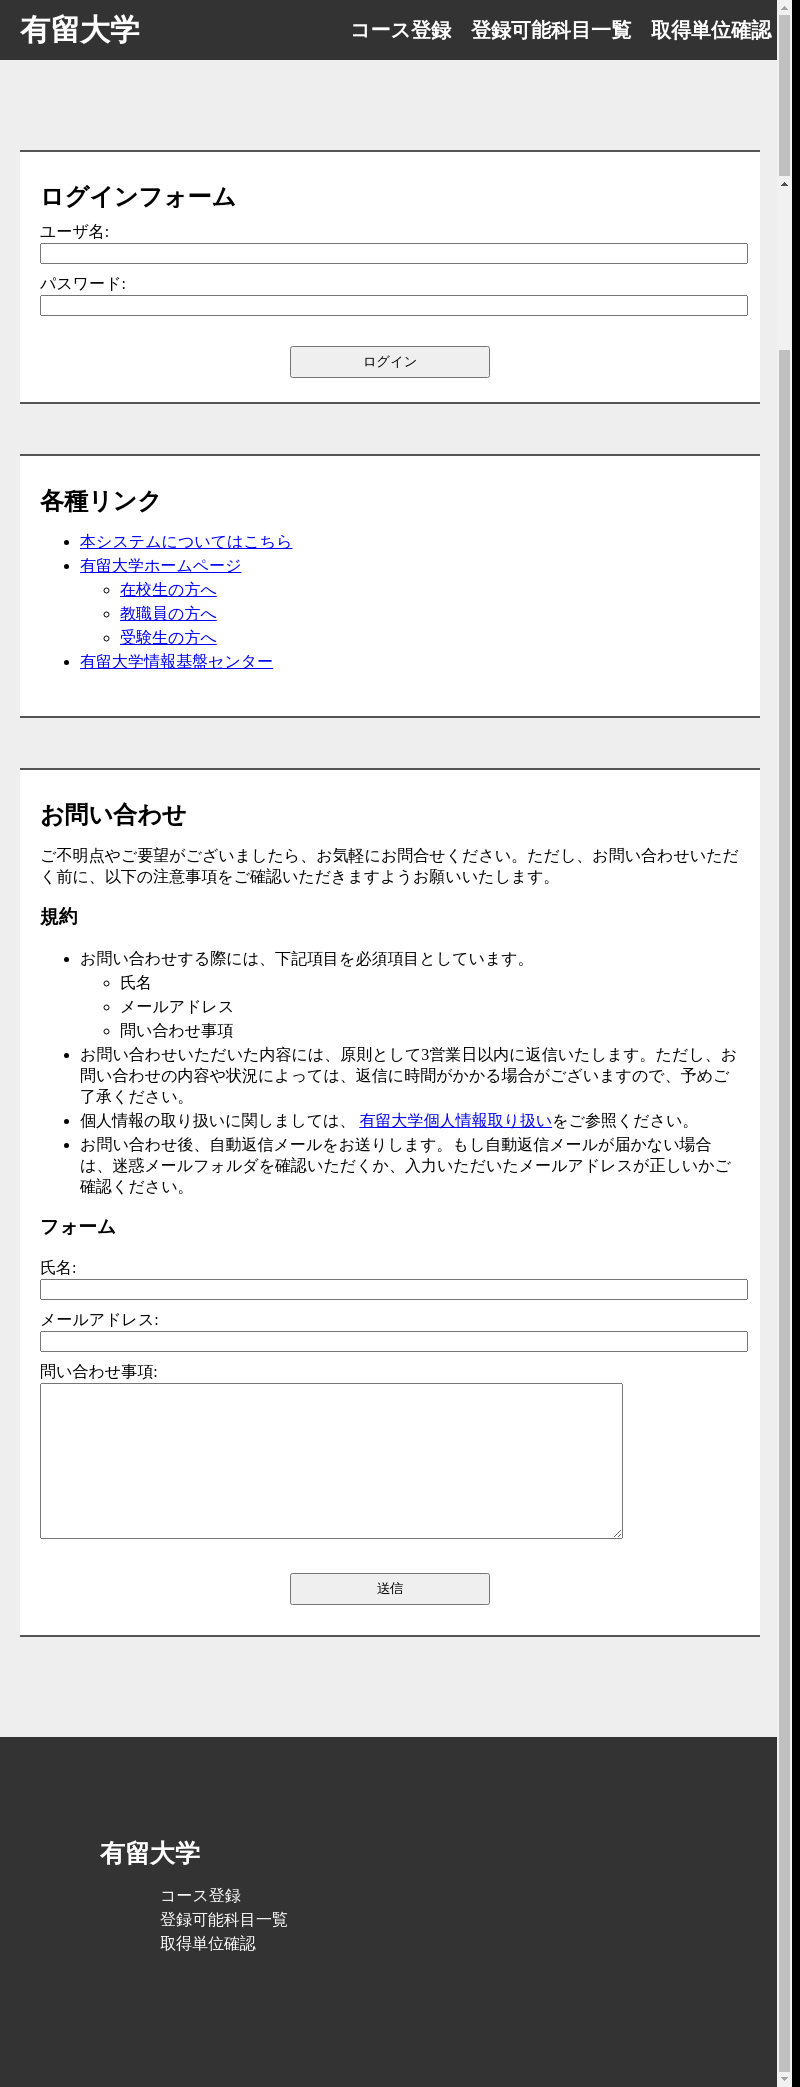
\includegraphics[width=0.5\textwidth]{image/5/original_png/bf_original.png}
    \caption{テスト対象とするWebページA}
    \label{fig:bf_original}
\end{figure}

\begin{figure}[htbp]
    \centering
    % 画像ファイル名とサイズを指定
    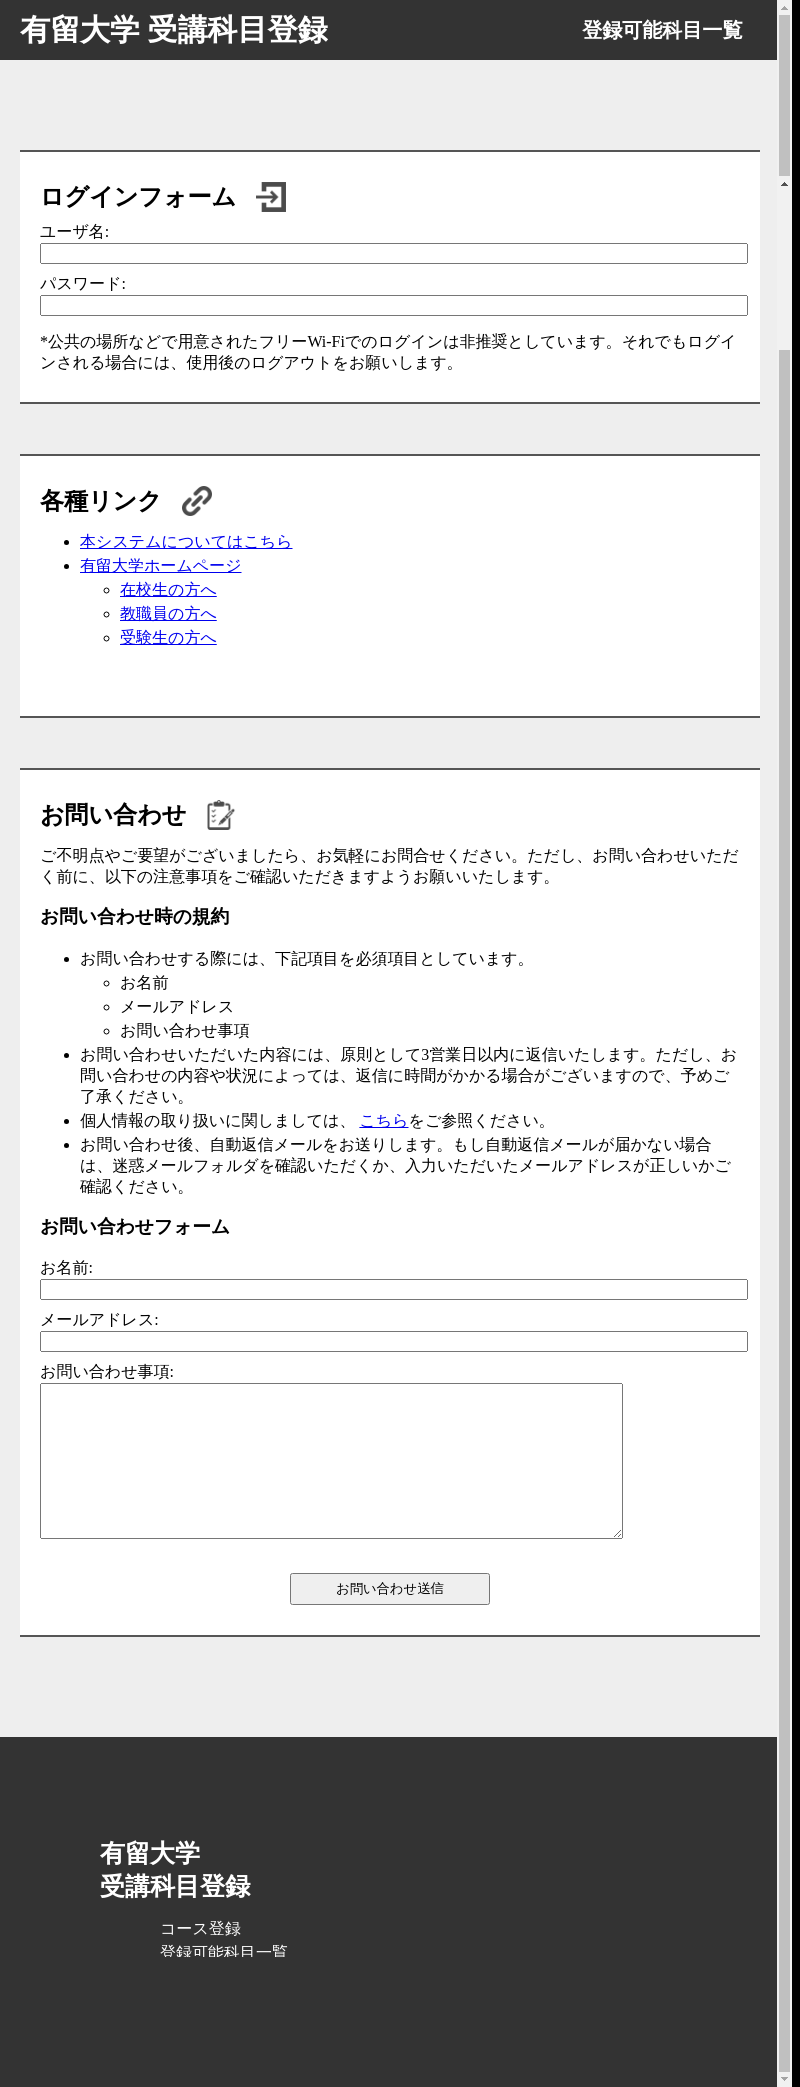
\includegraphics[width=0.5\textwidth]{image/5/original_png/af_original.png}
    \caption{図\ref{fig:bf_original}のWebページAにレイアウトの不具合が発生する変更を埋め込んだWebページB}
    \label{fig:af_original}
\end{figure}
上記のWebページを使用することで、
適用例に対して視覚的回帰テストを行った\toolName の各表示タブを確認することができる。

以降の節では、適用例を用いて、\toolName が持つ以下のそれぞれの機能について、確認する。
% 画像比較に基づく差分箇所表示、HTMLコードの変更に基づく変更箇所表示、レイアウトの不具合箇所表示
% のそれぞれの
% 画像比較に基づく差分箇所からHTMLコードに基づかないレイアウトの不具合箇所を
% 可視化できることを確認する。
% \toolName のUIは、以下に示す4つのタブを持つタブメニューと、各タブに対応するタブコンテンツからなる。
% \begin{itemize}
%     \item[①] タブメニュー
%           \begin{itemize}
%               \item オリジナル表示タブ
%               \item 画像比較に基づく差分箇所表示タブ
%               \item HTMLコードの変更に基づく変更箇所表示タブ
%               \item レイアウトの不具合箇所表示タブ
%           \end{itemize}
%     \item[②] タブコンテンツ
% \end{itemize}
% \par
% \toolName を用いて、HTMLコードに基づかないレイアウトの不具合箇所を可視化できるかどうかを確認するために、以下の4つのパターンについて確認する。
% \begin{itemize}
%     \item  画像比較に基づく差分箇所通りにHTMLコードに基づく変更箇所に削除されている
%     \item 画像比較に基づく差分箇所通りにHTMLコードに基づく変更箇所に削除されていない
%     \item 画像比較に基づく差分箇所通りにHTMLコードに基づく変更箇所に追加されている
%     \item 画像比較に基づく差分箇所通りにHTMLコードに基づく変更箇所に追加されていない
% \end{itemize}
% \par

\section{画像比較に基づく差分箇所表示の確認}
適用例を用いて、画像比較に基づく差分箇所表示が、正しく行われていることを確認する。
図\ref{fig:bf_original}と図\ref{fig:af_original}の適用例における画像の比較に基づく差分箇所表示を、図\ref{fig: 5_app2}に示す。
図\ref{fig: 5_app2}より、画像比較に基づく差分箇所表示が、正しく行われていることを確認できる。

\begin{figure}[tp]
    \begin{center}
        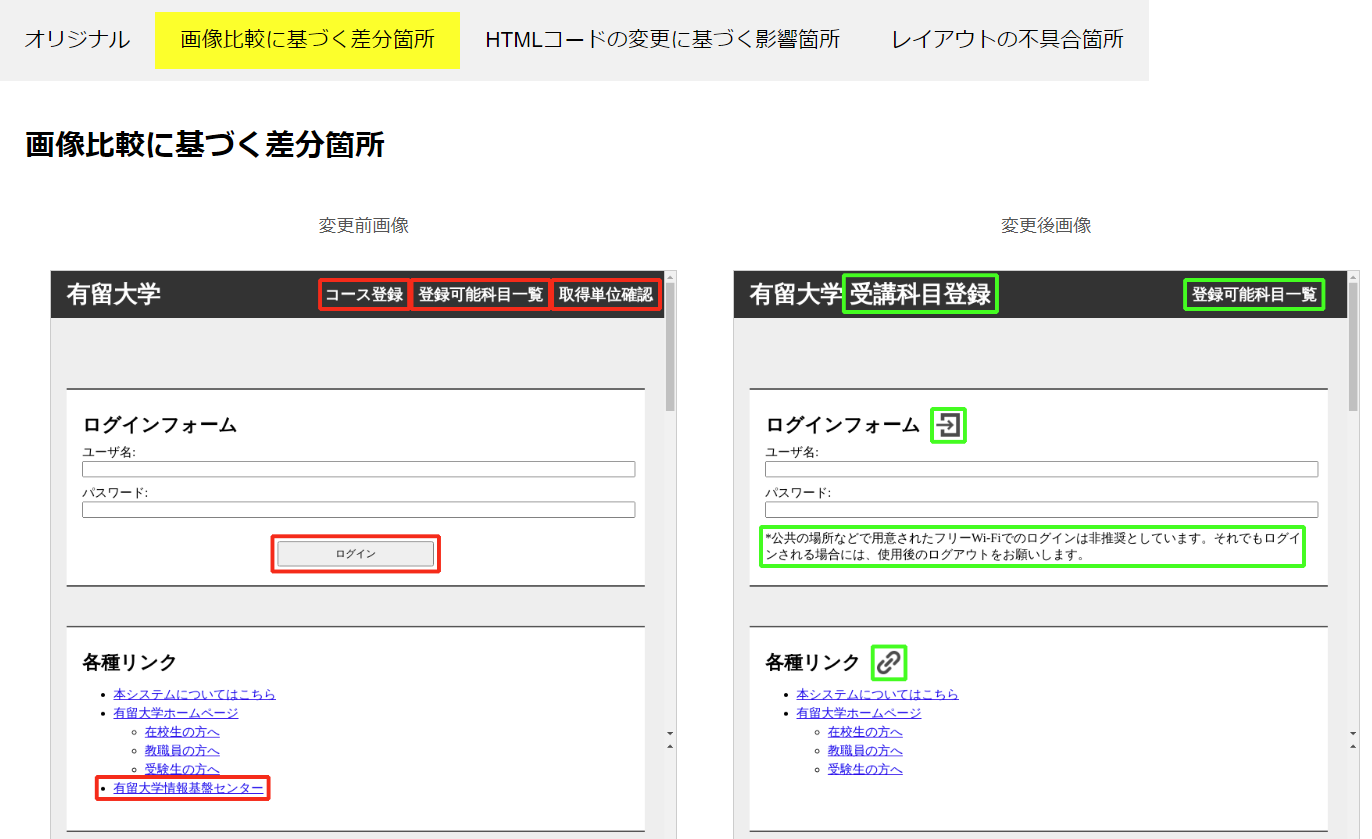
\includegraphics[width=1.0\columnwidth]{image/5/5_app2.png}
        \caption{図\ref{fig:bf_original}と図\ref{fig:af_original}における画像比較に基づく差分箇所表示}
        \label{fig: 5_app2}
    \end{center}
\end{figure}



\section{HTMLコードの変更に基づく変更箇所表示の確認}
適用例を用いて、HTMLコードの比較に基づく変更箇所表示が、正しく行われていることを確認する。
図\ref{fig:bf_original}と図\ref{fig:af_original}の適用例における変更箇所表示を、図\ref{fig: 5_app1}に示す。
図\ref{fig: 5_app1}より、HTMLコードの比較に基づく変更箇所表示が、正しく行われていることを確認できる。
\begin{figure}[tp]
    \begin{center}
        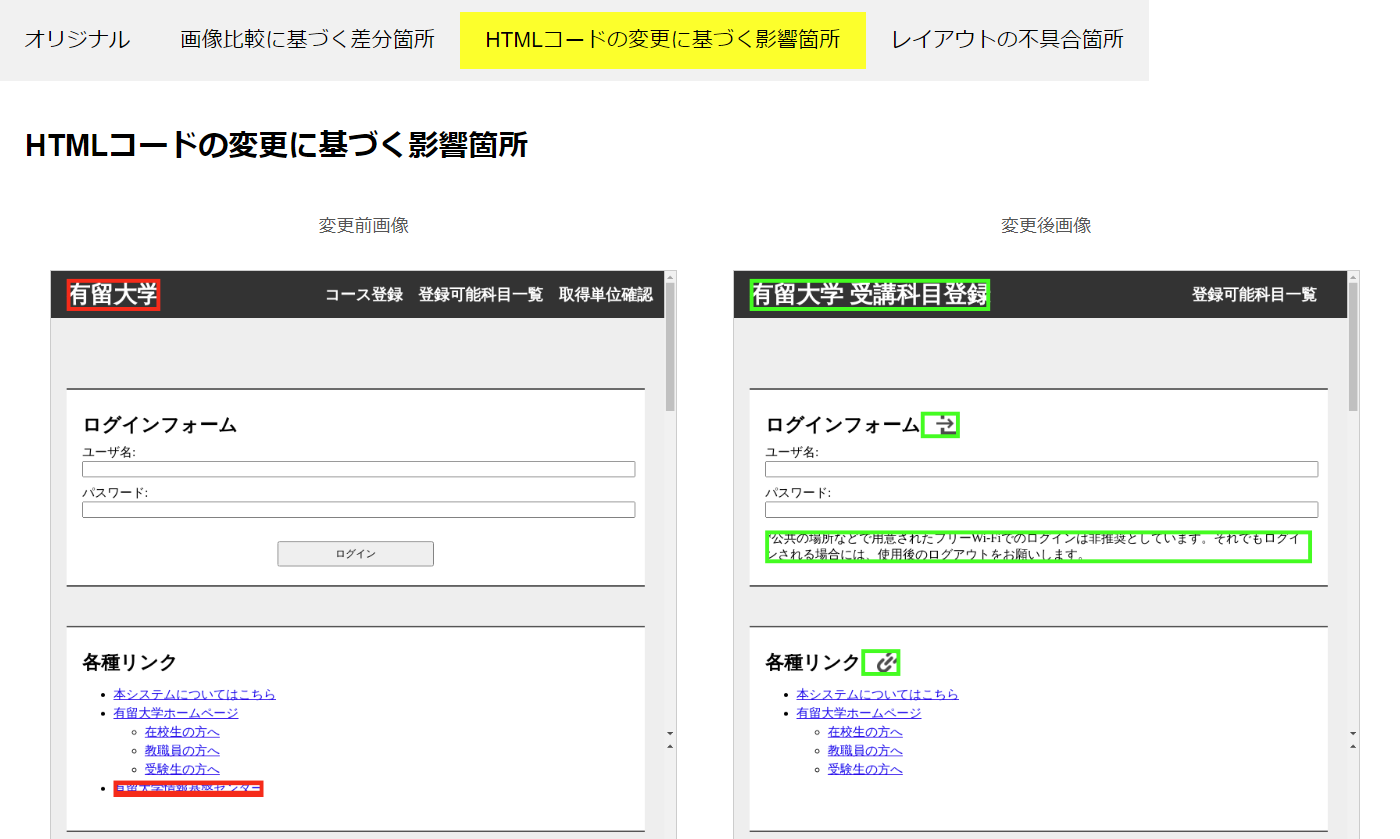
\includegraphics[width=1.0\columnwidth]{image/5/5_app1.png}
        \caption{図\ref{fig:bf_original}と図\ref{fig:af_original}の適用例における変更箇所表示}
        \label{fig: 5_app1}
    \end{center}
\end{figure}


\section{レイアウトの不具合箇所表示の確認}
適用例を用いて、レイアウトの不具合箇所表示が、正しく行われていることを確認する。
図\ref{fig:bf_original}と図\ref{fig:af_original}の適用例におけるレイアウトの不具合箇所表示を、図\ref{fig: 5_app3}に示す。
HTMLコードに基づかないレイアウトの不具合箇所を確認するために、以下の4つのパターンについて確認する。
\begin{itemize}
    \item 画像比較に基づく差分箇所通りにHTMLコードに基づく変更箇所に削除されている
    \item 画像比較に基づく差分箇所通りにHTMLコードに基づく変更箇所に削除されていない
    \item 画像比較に基づく差分箇所通りにHTMLコードに基づく変更箇所に追加されている
    \item 画像比較に基づく差分箇所通りにHTMLコードに基づく変更箇所に追加されていない
\end{itemize}
図\ref{fig: 5_app3}より、レイアウトの不具合箇所表示が、正しく行われていることを確認できる。
\begin{figure}[tp]
    \begin{center}
        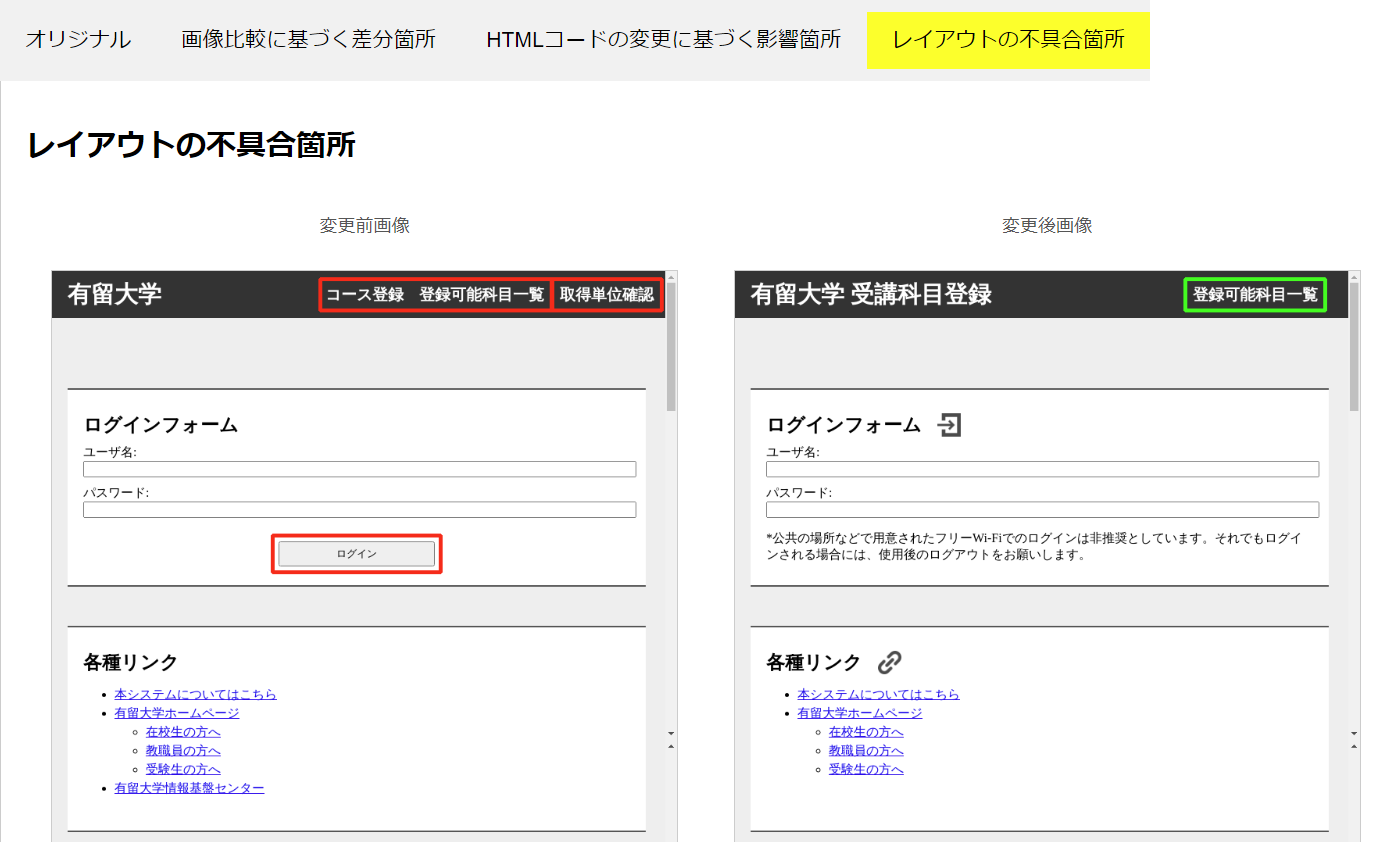
\includegraphics[width=1.0\columnwidth]{image/5/5_app_3.png}
        \caption{図\ref{fig:bf_original}と図\ref{fig:af_original}の適用例におけるレイアウトの不具合箇所表示}
        \label{fig: 5_app3}
    \end{center}
\end{figure}




\subsection{パターン1: 差分箇所通りに削除されている}\label{sec:result_area_detection}
適用例を用いて、差分箇所通りに削除されていることを確認する。
図\ref{fig: 5_app2}の画面を確認すると、変更前画像上の一番下のリンクが赤枠で囲まれていることが分かる。
この赤枠に着目すると、赤枠は変更後画像上で削除されていることが分かる。
次に、差分箇所通りに削除されているかどうかを確かめるために、
図\ref{fig: 5_app1}のHTMLコードの比較に基づく変更箇所表示タブを確認すると、
赤枠で囲まれているため、HTMLコードに基づいて削除された箇所だと分かる。
最後に、図\ref{fig: 5_app3}のレイアウトの不具合箇所表示タブで確認すると、
レイアウトの不具合箇所として赤枠で囲まれていないことが分かる。
\par
よって、\toolName は、差分箇所通りに削除されていることを確認できる。



\subsection{パターン2: 差分箇所通りに削除されていない}\label{sec:result_area2}
適用例を用いて、差分箇所通りに削除されていないことを確認する。
図\ref{fig: 5_app2}の画面を確認すると、変更前画像上のログインボタンが赤枠で囲まれていることが分かる。
この赤枠に着目すると、変更後画像上で削除されていることが分かる。
次に、差分箇所通りに削除されているかどうかを確かめるために、
図\ref{fig: 5_app1}のHTMLコードの比較に基づく変更箇所表示タブを確認すると、
赤枠で囲まれていないため、HTMLコードに基づいて削除されていない箇所だと分かる。
このことから、緑枠で囲まれたテキストによって、ログインボタンが隠れた状態になっていると推測できる。
最後に、図\ref{fig: 5_app3}のレイアウトの不具合箇所表示タブで確認すると、
レイアウトの不具合箇所として赤枠で囲まれていることが分かる。
\par
よって、\toolName は、差分箇所通りに削除されていないことを確認できた。


\subsection{パターン3: 差分箇所通りに追加されている}\label{sec:result_area3}
適用例を用いて、差分箇所通りに追加されていることを確認する。
図\ref{fig: 5_app2}の画面を確認すると、変更後画像上の左上テキスト「受講科目登録」が緑枠で囲まれていることが分かる。
この緑枠に着目すると、変更前画像上から追加されていることが分かる。
次に、差分箇所通りに追加されているかどうかを確かめるために、
図\ref{fig: 5_app1}のHTMLコードの比較に基づく変更箇所表示タブを確認すると、
緑枠で囲まれているため、HTMLコードに基づいて追加された箇所だと分かる。
最後に、図\ref{fig: 5_app3}のレイアウトの不具合箇所表示タブで確認すると、
レイアウトの不具合箇所として緑枠で囲まれていないことが分かる。
\par
よって、\toolName は、差分箇所通りに追加されていることを確認できた。


\subsection{パターン4: 差分箇所通りに追加されていない}\label{sec:result_area4}
適用例を用いて、差分箇所通りに追加されていないことを確認する。
図\ref{fig: 5_app2}の画面を確認すると、変更後画像上の右上テキスト「登録可能科目一覧」が緑枠で囲まれていることが分かる。
この緑枠に着目すると、緑枠内のテキストと完全一致するテキストが変更前画像上に赤枠で囲まれているため、
変更前画像上から削除され、変更後画像上に新しく追加されていることが分かる。
% つまり、変更後にテキストの配置の変更があったと推測できる。
次に、差分箇所通りに追加されているかどうかを確かめるために、
図\ref{fig: 5_app1}のHTMLコードの比較に基づく変更箇所表示タブを確認すると、
緑枠で囲まれていないため、HTMLコードに基づいて追加されていない箇所だと分かる。
最後に、図\ref{fig: 5_app3}のレイアウトの不具合箇所表示タブで確認すると、
レイアウトの不具合箇所として緑枠で囲まれていることが分かる。
\par
よって、\toolName は、差分箇所通りに削除されていないことを確認できた。
% \section{画面要素の隠れが発生したWebページ}\label{subsec:result_rect_area}
% \subsection{Case1:開発者の意図しないレイアウトの不具合}\label{subsec:result_rect_area}

% \subsection{Case2:開発者が意図して画面要素を消した場合}\label{subsec:result_underline_area}

% \subsection{Case3:開発者が意図せず画面要素を消した場合}\label{subsec:result_underline}


% \section{画面要素の見切れが発生したWebページ}\label{subsec:result_underline_area}
% \subsection{Case1:開発者の意図しないレイアウトの不具合}\label{subsec:result_rect_area}

% \subsection{Case2:開発者が意図して画面要素を消した場合}\label{subsec:result_underline_area}

% \subsection{Case3:開発者が意図せず画面要素を消した場合}\label{subsec:result_underline}

% \section{画面要素の重なりが発生したWebページ}\label{sec:result_area_detection}

% \subsection{Case1:開発者の意図しないレイアウトの不具合}\label{subsec:result_rect_area}

% \subsection{Case2:開発者が意図して画面要素を消した場合}\label{subsec:result_underline_area}

% \subsection{Case3:開発者が意図せず画面要素を消した場合}\label{subsec:result_underline}
\chapter{考察}\label{cha:discussion}
本研究では、レイアウトの不具合箇所の発見にかかる時間の削減を目的として、
レイアウトの不具合箇所を強調表示する視覚的回帰テストツール\toolName(Mix Visual Regression Testing)を試作した。
本章では、
評価実験を行い、\toolName の有用性を評価する。
次に、\toolName と関連研究を比較する。
最後に、\toolName の問題点とその解決策について述べる。

\section{評価実験}
評価実験では、レイアウトの不具合箇所の発見にかかる時間に対する評価を行う。
具体的には、\toolName を使用した場合と、従来の画像ベースの視覚的回帰テストで生成する差分画像を使用する場合とで、
レイアウトの不具合箇所の発見にかかる時間を、それぞれ計測する。

\toolName を使用する場合では、
\toolName の実行完了後から、被験者がレイアウトの不具合箇所を見つけるまでにかかった時間を発見時間として計測する。
従来手法では、
\toolName の画像比較に基づく差分箇所表示を見てから、被験者がレイアウトの不具合箇所を見つけるまでにかかった時間を発見時間として計測する。

実験の事前準備として、HTMLコードで記述された実験用Webページを$\alpha$と$\beta$の2つ作成し、それぞれ変更前と変更後のHTMLコードを用意する。
なお、2つの実験用Webページについて、変更後のWebページには、それぞれ3個のレイアウトの不具合箇所を埋め込む。
Webページ$\alpha$は、架空の大学についてのWebページである。
Webページ$\beta$は、架空のツールを紹介するWebページである。
実験に使用するWebページ$\alpha$の変更前画像と変更後画像を図\ref{fig:test1}に、
実験に使用するWebページ$\beta$の変更前画像と変更後画像を図\ref{fig:test2}に
示す。
\begin{figure}[tp]
    \centering
    % 画像ファイル名とサイズを指定
    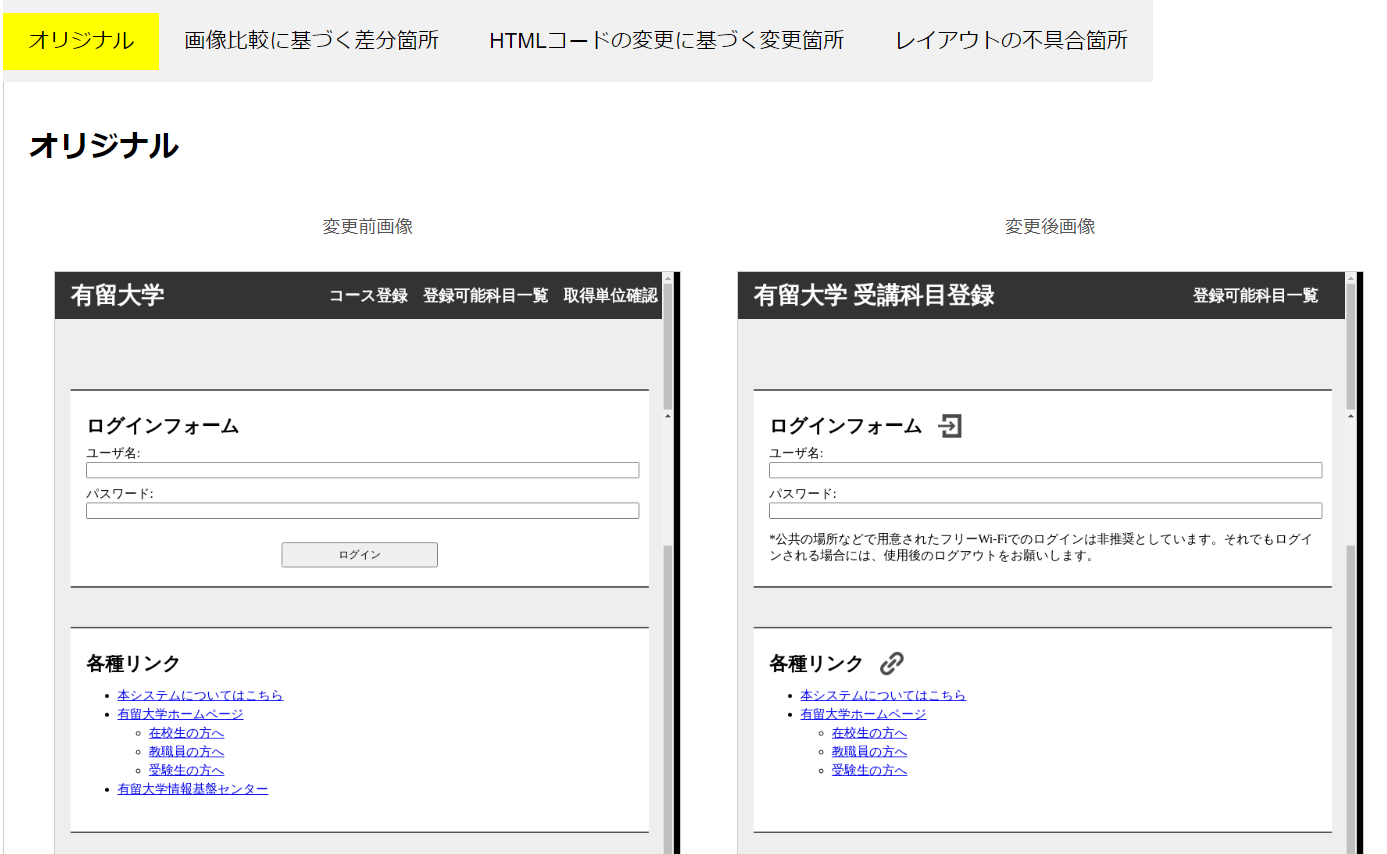
\includegraphics[width=1.0\textwidth]{image/5/new_original.png}
    \caption{実験に使用するWebページ$\alpha$の変更前画像と変更後画像}
    \label{fig:test1}
\end{figure}
\begin{figure}[tp]
    \centering
    % 画像ファイル名とサイズを指定
    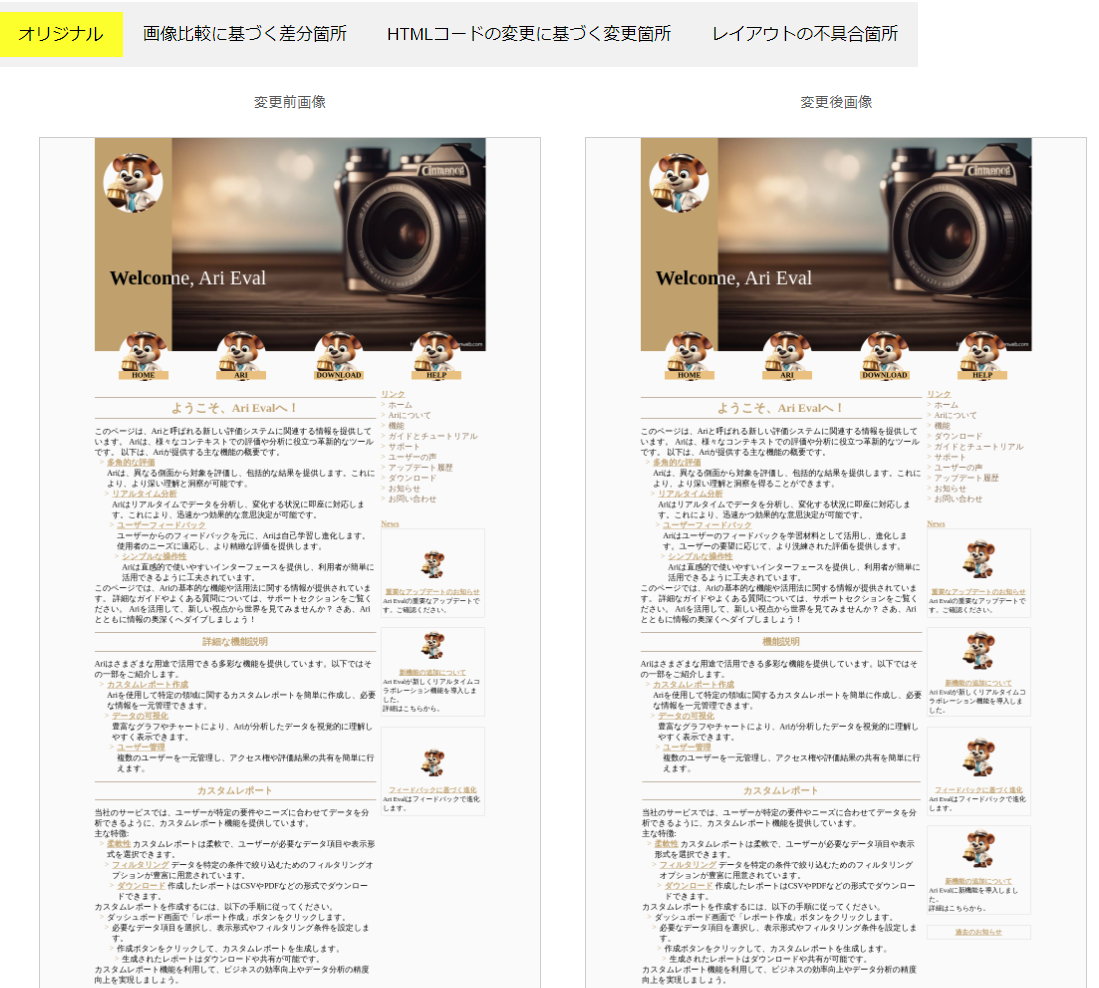
\includegraphics[width=1.0\textwidth]{image/6/test_beta.png}
    \caption{実験に使用するWebページ$\beta$の変更前画像と変更後画像}
    \label{fig:test2}
\end{figure}
実験に参加する被験者は、宮崎大学で情報工学を専攻する4人の学生(以降、被験者A~Dと呼ぶ)である。
実験を行う際には、実験用Webページの変更前画像と変更後画像を見ることができ、
また、実験用Webページの変更前HTMLコードと変更後HTMLコードも見ることができる。
さらに、被験者がレイアウトの不具合箇所を見つけた際に、その不具合箇所の位置を記録しておくための実験用ファイルも用意する。
% 被験者の中には、Webに関する知識がない者も含まれるが、今回は事前に説明する。
% 実験では、【実験によって\toolName が達成したいことを満たせているかを確認するためにこのような作業を提示する】。
% 以降、各作業の内容と結果を説明する。
\par
\toolName を使用する場合では被験者は、図\ref{fig:test1_subeffect}に示した
\toolName のレイアウトの不具合箇所表示を用いて、
レイアウトの不具合箇所を確認する。
確認したレイアウトの不具合箇所は実験用ファイルに書き込んでもらい、被験者が全てのレイアウトの不具合箇所を見つけたと判断したら実験を終了する。
\begin{figure}[tp]
    \centering
    % 画像ファイル名とサイズを指定
    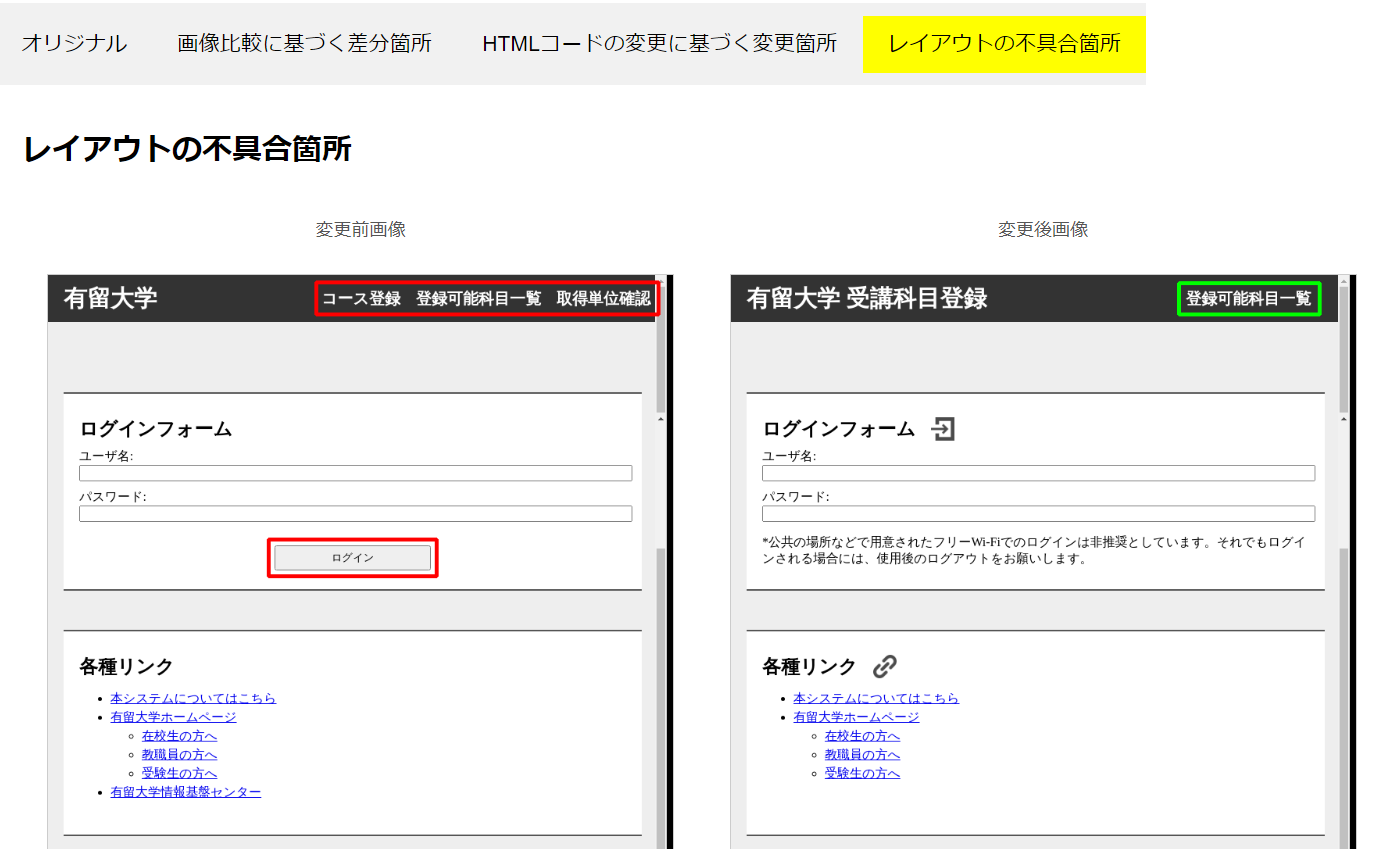
\includegraphics[width=1.0\textwidth]{image/5/new_effect.png}
    \caption{Webページ$\alpha$におけるレイアウトの不具合箇所表示}
    \label{fig:test1_subeffect}
\end{figure}

従来手法では被験者は、図\ref{fig:test1_img}に示した\toolName の画像比較に基づく差分箇所表示を用いて、
レイアウトの不具合箇所を見つける。また、実験用Webページの変更前HTMLコードと変更後HTMLコードも確認することで、
画像比較に基づく差分箇所が、レイアウトの不具合箇所であるかどうかを判定する。
見つけたレイアウトの不具合箇所は実験用ファイルに書き込んでもらい、被験者が全てのレイアウトの不具合箇所を見つけたと判断したら実験を終了する。
\begin{figure}[tp]
    \centering
    % 画像ファイル名とサイズを指定
    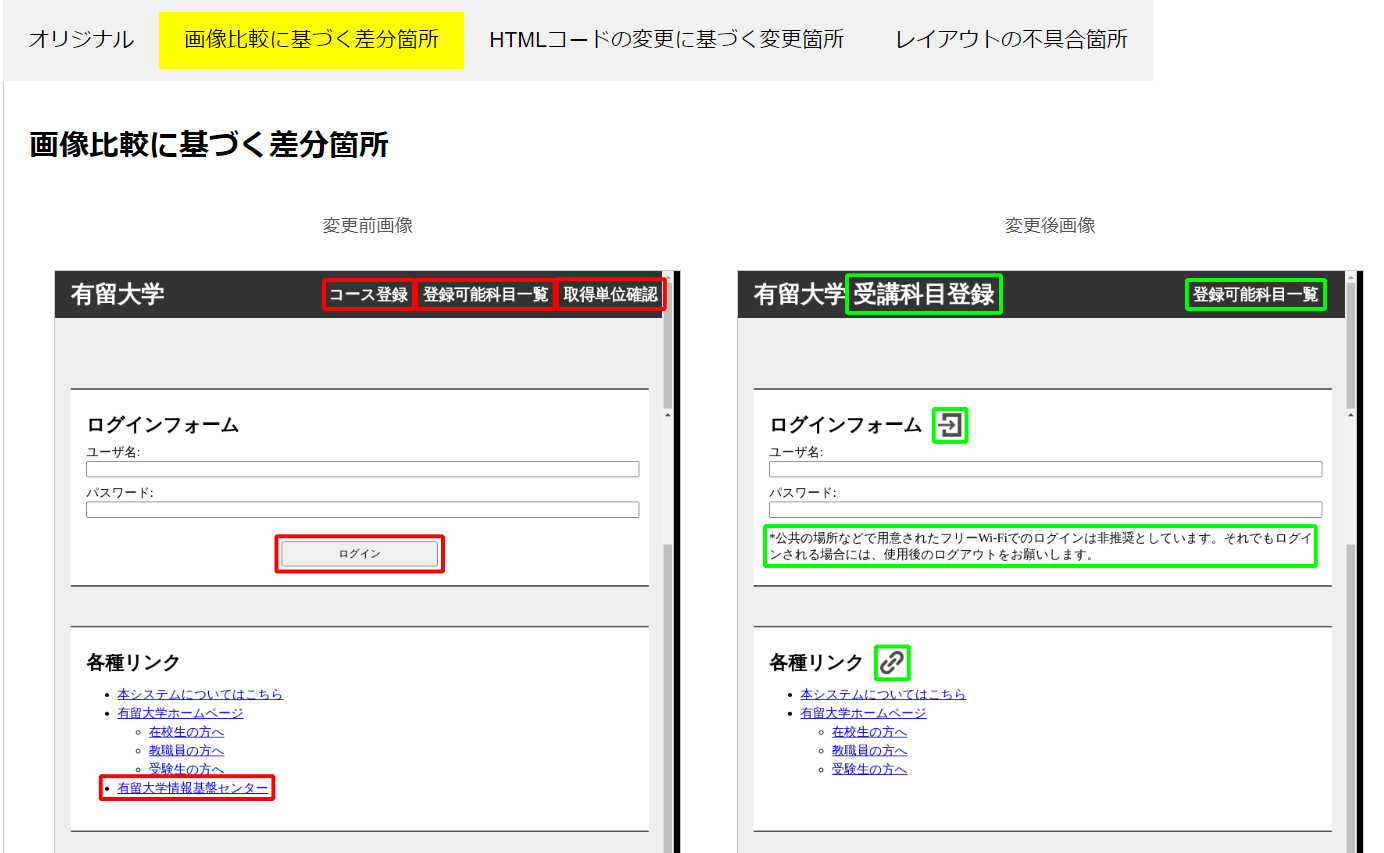
\includegraphics[width=1.0\textwidth]{image/5/new_img.png}
    \caption{Webページ$\alpha$における画像比較に基づく差分箇所表示}
    \label{fig:test1_img}
\end{figure}
従来手法におけるレイアウトの不具合箇所を見つける流れについて、以下に示す。
\begin{enumerate}
    \item 画像比較に基づく差分箇所表示で、変更前画像上の全ての赤枠に対して、以下の操作を繰り返す。
          \begin{enumerate}
              \item 赤枠内の画面要素が、実験用Webページの変更後HTMLコードに存在しない、または、CSSクラスが変更されている場合、その画面要素は削除、または、変更されたと判定し、次の赤枠の確認に進む。
              \item 上記以外の場合、その画面要素は削除されていないと判定する。この場合、レイアウトの不具合箇所であるため、実験用ファイルに記録を取る。
          \end{enumerate}
    \item 画像比較に基づく差分箇所表示で、変更後画像上の全ての緑枠に対して、以下の判定を繰り返す。
          \begin{enumerate}
              \item 緑枠内の画面要素が、実験用Webページの変更前HTMLコードに存在しない、または、CSSクラスが変更されている場合、その画面要素は追加されたと判定し、次の緑枠の確認に進む。
              \item 上記以外の場合、その画面要素は追加されていないと判定する。この場合、レイアウトの不具合箇所であるため、実験用ファイルに記録を取る。
          \end{enumerate}
\end{enumerate}


\section{レイアウトの不具合箇所の発見時間に関する評価}\label{subsec:evalue_required_time}
レイアウトの不具合箇所を発見するのにかかった時間についての実験結果を、表\ref{fig: 6_1}に示す。
% 被験者Aは、大学ページを手動で16m 16s、Ariをツールで39s。
% 被験者Bは、大学ページをツールで1m 3s、Ariを手動で13m 40s。
% 被験者$\alpha$は、大学ページを手動で11m 54s、Ariをツールで48s。
% 被験者$\beta$は、大学ページをツールで2m 37s、Ariを手動で12m 45s。

表\ref{fig: 6_1}から、\toolName を使用することで、発見時間を平均で12分22秒(90.6\%)削減することができた。
このことから、\toolName を用いた視覚的回帰テストでは、
レイアウトの変更が生じた箇所に対して、
HTMLコードを確認してレイアウトの不具合箇所であるかどうかを確認する手間を削減できたといえる。
よって、\toolName は、レイアウトの不具合箇所の発見にかかる時間の削減に有用である。

\begin{table}[tp]
    \centering
    \caption{レイアウトの不具合箇所の発見時間についての実験結果}
    \label{fig: 6_1}
    \begin{tabular}{c||c|c|c|c}
               & \multicolumn{2}{|c|}{\textbf{Webページ$\alpha$}}
               & \multicolumn{2}{|c}{\textbf{Webページ$\beta$}}                                      \\
        \hline \hline
        被験者 & \toolName                                        & 従来手法 & \toolName & 従来手法  \\
        \hline \hline
        A      & -                                                & 16m 16s  & 39s       & -         \\
        B      & -                                                & 11m 54s  & 48s       & -         \\
        C      & 1m 3s                                            & -        & -         & 13m 40s   \\
        D      & 2m 37s                                           & -        & -         & 12m 5s    \\
        \hline
        平均   & 1m 50s                                           & 14m 5s   & 43.5s     & 13m 12.5s \\
    \end{tabular}
\end{table}


\section{レイアウトの不具合箇所の検出精度に関する評価}\label{subsec:evalue_accuracy}
評価実験において、従来手法では、被験者が
レイアウトの不具合箇所を過剰に検出することや、検出が不足することがあった。
それに対して、\toolName を用いることで、
レイアウトの不具合箇所を過不足なく検出できた。

従来手法におけるレイアウトの不具合箇所を過剰に検出した数と、検出が不足した数を、表\ref{tb:result_detect}に示す。
なお、表\ref{tb:result_detect}における不具合箇所は、Webページ$\alpha$と$\beta$にそれぞれ加えたレイアウトの不具合箇所の総数を意味する。
\begin{table}[tp]
    \centering
    \caption{従来手法におけるレイアウトの不具合箇所を過剰に検出した数と検出が不足した数}
    \label{tb:result_detect}
    \begin{tabular}{c||c|c|c|c|c}
        Webページ                 & 不具合箇所         & 被験者 & 過剰 & 不足 & \\
        \hline \hline
        \multirow{2}{*}{$\alpha$} & \multirow{2}{*}{3} & A      & 0    & 0    & \\
        \cline{3-6}
                                  &                    & B      & 0    & 2    & \\
        \hline
        \multirow{2}{*}{$\beta$}  & \multirow{2}{*}{3} & C      & 1    & 1    & \\
        \cline{3-6}
                                  &                    & D      & 2    & 1    & \\
        \hline \hline
    \end{tabular}
\end{table}

従来手法で被験者がレイアウトの不具合箇所を過剰に検出したことについて、考察する。
被験者CとDは、
見た目の変更があった画面要素に対して、HTMLコードに基づく変更がされていたかどうかの
判定を誤ったため、レイアウトの不具合箇所を過剰に検出したと考える。
判定を誤った箇所の変更後の差分画像を、図\ref{fig:app1}に示す。
また、判定を誤った箇所の変更前のHTMLコードによる変更箇所を、図\ref{fig:app2}に示す。
判定を誤った原因として、
画像比較による差分画像では、図\ref{fig:app1}に示すように、「カスタムレポート」は囲まれておらず、
HTMLコードに基づく変更箇所では、図\ref{fig:app2}に示すように「カスタムレポート」が囲まれている。
これにより、差分画像しか用いない従来手法では、実際の変更箇所を発見することが困難であるため、
レイアウトの不具合箇所であると誤って判定してしまったと考える。
\begin{figure}[tp]
    \centering
    % 画像ファイル名とサイズを指定
    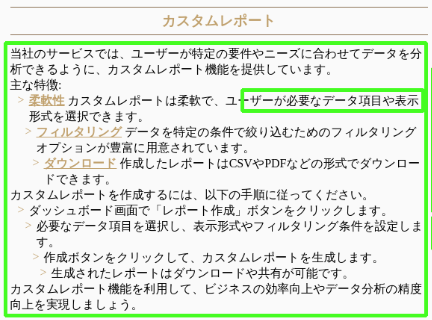
\includegraphics[width=1.0\textwidth]{image/6/miss_af_img.png}
    \caption{Webページ$\beta$において判定を誤った箇所の変更後の差分画像}
    \label{fig:app1}
\end{figure}

\begin{figure}[tp]
    \centering
    % 画像ファイル名とサイズを指定
    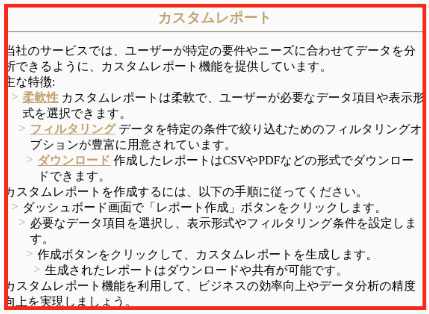
\includegraphics[width=1.0\textwidth]{image/6/miss_bf_html.png}
    \caption{Webページ$\beta$において判定を誤った箇所の変更前のHTMLコードによる変更箇所}
    \label{fig:app2}
\end{figure}

従来手法を用いた被験者が検出できなかったレイアウトの不具合箇所について、考察する。
BからDの被験者らは、レイアウトの不具合箇所として加えた画面要素のはみ出しに対して、
レイアウトの不具合箇所の検出不足があった。このことから、
画面要素のはみ出しのような見た目だけで変更が分かりづらい差分があった場合は、従来の画像ベースの視覚的回帰テストでは検出しづらいことが分かった。

以上のことから、\toolName は、従来の画像ベースの視覚的回帰テストと比較して、
レイアウトの不具合箇所の発見に有用である。

\section{関連研究}\label{sec:relation_research}
本研究で試作した\toolName と、関連研究を比較する。
Daruto Tannoらは、領域ベースにおける視覚的回帰テストを行った\cite{RegionDetect}。
領域ベースで画像比較することで、本質的な差分と本質的でない差分を含んだ差分画像から、
本質的な差分のみを抽出できることを提案している。
また、塚越らは、GUI要素の階層構造を利用した差分検出方法を提案した\cite{GuiRetrExternal}。
\par
これらの既存研究は、手動で視覚的回帰テストを行う場合よりも、
画像比較による視覚的回帰テストを用いることにより、
レイアウトの不具合がないかどうかを効率的に見つけ出すことを提案している。
しかし、比較には画像のみを用いるため、抽出した差分が開発者の意図した変更かどうか判断できない。
そのため、HTMLコードの差分とレイアウトの差分との間の整合性の確認に時間がかかる。

これに対して、\toolName は、画像比較に基づく差分箇所から、HTMLコードの変更に基づく変更箇所を除いた、
レイアウトの不具合箇所のみを強調表示することができる。
そのため、\toolName は、既存研究と比較して、レイアウトの不具合箇所の発見に
有用であるといえる。

\section{\toolName の問題点とその解決策}\label{sec:AWSAL_problems}
\toolName の問題点とその解決策について、以下に示す。
\begin{itemize}
    \item テスト対象とするWebページの画面サイズにおける問題:\\
          テスト対象とする変更前後のWebページの画面サイズが同じでないと、
          視覚的回帰テストを行うことができない。変更前後のWebページの画面サイズが異なる場合は、画面サイズの差に閾値を設定することで、
          その閾値以内なら、画像の調整や比較方法を動的に変更できるようにする必要がある。
    \item 画像比較の制限に関する問題:\\
          現在の\toolName では、一度の実行で1回しかテストできない。このため、多くのWebページをテストする必要があるWebサイトに有用性があると言えない。
          テスト対象とするWebページだけでなく、サイト内の全てのWebページに対しても、視覚的回帰テストを行えるようにしなければ、
          実用的だと言えない。解決策として、Seleniumによるスクレイピング技術を用いたり、開発リポジトリをクローンしておくだけでそのリポジトリにおける開発Webページに対して、
          視覚的回帰テストを自動で実行できる機能を実装する必要がある。
    \item 入力対象とするWebページの背景における問題:\\
          背景が白地でなく、赤色や緑色であったりした場合に、適切に変更箇所に色付きの枠を付けることができない。
          現在の\toolName では、HTMLの変更箇所に赤枠や緑枠をつけて強調表示したり、画像比較で生成した差分画像に赤枠や緑枠をつけて強調表示したりしている。
          このため、
          テスト対象とするWebページの背景が白地でなく、赤や緑など強調する色付きの枠と同じであると、適切に画像を強調することができない。
          解決策として、そのようなWebページは視覚的回帰テストの対象としない処理にするか、背景の色や画像内に多く含む色を検出し、その色と区別できる色で変更箇所を強調表示する必要があると考える。
    \item 入力対象とするWebページのHTML構造における問題:\\
          現在の\toolName では、HTML構造が一定の形式に沿っていないと適切にHTMLを解析することができず、開発者の意図した変更箇所を適切に囲まない枠付きHTMLコードを生成してしまう。
          この解決策として、HTMLコードの解析をテキストベースで行うのではなく、DOM解析やより高度な解析技術を用いて、HTMLコードの解析が必要となる。
    \item HTMLコード以外のファイル取得における問題:\\
          画像取得部によるHTMLコードの取得では、取得するHTMLコードのCSSやJavaScriptが別ファイルで記述されていると、そのファイルを読み込むことができず、適切な枠付きHTMLコードを生成できない。解決策として、
          単一のHTMLコードだけでなく、そのHTMLに用いるCSSやJavascriptのファイルも取得できるようにする必要がある。
    \item レイアウトの不具合箇所の検出方法における問題:\\
          現在の\toolName では、親子関係にある画面要素間に重なりが発生しても、その箇所をレイアウトの不具合箇所として強調表示することができない。
          これが起こる原因は、レイアウトの不具合箇所を検出する際に、
          差分箇所に付ける枠と変更箇所に付ける枠の重なりを比較し、重なりの面積が小さい方の面積の5割以上の場合に、それらの枠を意図的な差分と判定する。
          親子関係にある画面要素は、親要素が子要素を完全に内包していることが多いため、これらをレイアウトの不具合箇所として検出できない。
          解決策として、画像内にある枠の構造化を行い、親要素が子要素を完全に内容している場合は、別途処理を行う必要がある。
\end{itemize}

\chapter{おわりに}\label{cha:Conclusion}
本研究では、Webページのレイアウトの不具合箇所の発見にかかる時間の削減を目的として、
Webページのレイアウト不具合箇所を強調表示する視覚的回帰テストツール\toolName(Mix Visual Regression Testing)を試作した。
\par
\toolName は、以下の3つを強調表示する機能を持つ。
\begin{itemize}
      \item 差分箇所:\\
            変更前後のWebページの画像を比較して、変更前のWebページから削除された範囲と、
            変更後のWebページに追加された範囲。
      \item 変更箇所:\\
            変更前後のWebページのHTMLコードを比較して、HTMLコードにおけるbody要素内の変更とstyle要素内の変更のどちらか、
            または両方が適用された画面要素の範囲。
            本研究では、変更箇所を意図的なレイアウトの差分の範囲とみなす。
      \item レイアウトの不具合箇所:\\
            差分箇所から、意図的なレイアウトの差分の範囲であるHTMLコードの変更箇所を除いた、
            レイアウトの不具合の範囲。
\end{itemize}
\par
以下の4つのケースに対して、\toolName を用いて視覚的回帰テストを実行することで、レイアウトの不具合箇所を強調表示できることを確認した。
\begin{enumerate}[label=ケース\arabic*., leftmargin=1.8cm]
      \setlength{\itemsep}{0pt}
            \setlength{\parsep}{0pt}
      \item 画像比較に基づく差分箇所表示通りに画面要素が削除されており、レイアウトの不具合ではない
      \item 画像比較に基づく差分箇所表示通りには画面要素が削除されておらず、レイアウトの不具合である
      \item 画像比較に基づく差分箇所表示通りに画面要素が追加されており、レイアウトの不具合ではない
      \item 画像比較に基づく差分箇所表示通りには画面要素が追加されておらず、レイアウトの不具合である
\end{enumerate}
% 【下記は2章に書く】\\
% 画像比較に基づく差分箇所には、意図したレイアウトの変更と意図しないレイアウトの変更がある。
% 意図したレイアウトの変更はHTMLコードに基づいており、意図しないレイアウトの変更はHTMLコードに基づいていない。
% なお、本研究では、意図しないレイアウトの変更箇所を、「レイアウトの不具合箇所」と定義する。
\par
また、評価実験として、
\toolName を使用した場合と、
従来の画像ベースの視覚的回帰テストで生成する差分画像を使用する場合とで、レイアウトの不具合箇所の発見にかかる時間を、それぞれ計測した。
評価実験の結果、レイアウトの不具合箇所を発見するのにかかる時間を、
\toolName は、従来手法と比べて、
Webページ1つあたり平均で12分22秒(90.6\%)削減することができた。
さらに、\toolName は、すべてのレイアウトの不具合箇所を過不足なく検出できた。
一方、従来手法では、レイアウトの不具合箇所を過剰に検出することや、検出が不足することがあった。
この結果から、\toolName は、従来の画像ベースの視覚的回帰テストと比較して、
レイアウトの不具合箇所の発見に有用であることを確認した。
\par
以上のことから、本研究で試作した \toolName は、
レイアウトの不具合箇所の発見にかかる時間の削減に有用であるといえる。
\par
以下に、\toolName の今後の課題を示す。
\begin{itemize}
      \setlength{\itemsep}{0pt}
            \setlength{\parsep}{0pt}
      \item 画像サイズの差に対する閾値の設定:\\
            テスト対象とする変更前後のWebページの画面サイズが同じでないと、
            視覚的回帰テストを行うことができない。変更前後のWebページの画面サイズが異なる場合は、画面サイズの差に閾値を設定することで、
            その閾値以内なら、画像の調整や比較方法を動的に変更できるようにする必要がある。
      \item 画像比較の回数に対する拡張:\\
            現在の\toolName では、一度の実行で1回しかテストできない。このため、多くのWebページをテストする必要があるWebサイトに有用性があると言えない。
            テスト対象とするWebページだけでなく、サイト内の全てのWebページに対しても、視覚的回帰テストを行えるようにしなければ、
            実用的だと言えない。解決策として、Seleniumによるスクレイピング技術を用いたり、開発リポジトリをクローンしておくだけでそのリポジトリにおける開発Webページに対して、
            視覚的回帰テストを自動で実行できる機能を実装する必要がある。
      \item 白地以外の背景画像に対応する拡張:\\
            現在の\toolName では、HTMLの変更箇所に赤枠や緑枠をつけて強調表示したり、画像比較で生成した差分画像に赤枠や緑枠をつけて強調表示したりしている。
            このため、
            テスト対象とするWebページの背景が白地でなく、赤や緑など強調する色付きの枠と同じであると、適切に画像を強調することができない。
            解決策として、そのようなWebページは視覚的回帰テストの対象としない処理にするか、背景の色や画像内に多く含む色を検出し、その色と区別できる色で変更箇所を強調表示する必要があると考える。
      \item HTMLコード解析方法の変更による拡張:\\
            現在の\toolName では、HTML構造が一定の形式に沿っていないと適切にHTMLを解析することができず、開発者の意図した変更箇所を適切に囲まない枠付きHTMLコードを生成してしまう。
            この解決策として、HTMLコードの解析をテキストベースで行うのではなく、DOM解析やより高度な解析技術を用いて、HTMLコードの解析が必要となる。
      \item HTMLコード以外のファイル取得による拡張:\\
            画像取得部によるHTMLコードの取得では、取得するHTMLコードのCSSやJavaScriptが別ファイルで記述されていると、そのファイルを読み込むことができず、適切な枠付きHTMLコードを生成できない。解決策として、
            単一のHTMLコードだけでなく、そのHTMLに用いるCSSやJavascriptのファイルも取得できるようにする必要がある。
      \item レイアウトの不具合箇所の検出アルゴリズムの拡張:\\
            現在の\toolName では、親子関係にある画面要素間に重なりが発生しても、その箇所をレイアウトの不具合箇所として強調表示することができない。
            これが起こる原因は、レイアウトの不具合箇所を検出する際に、
            差分箇所に付ける枠と変更箇所に付ける枠の重なりを比較し、重なりの面積が小さい方の面積の5割以上の場合に、それらの枠を意図的な差分と判定する。
            親子関係にある画面要素は、親要素が子要素を完全に内包していることが多いため、これらをレイアウトの不具合箇所として検出できない。
            解決策として、画像内にある枠の構造化を行い、親要素が子要素を完全に内容している場合は、別途処理を行う必要がある。
\end{itemize}

% \par
% 初期設定を行った状態でテスト対象とするWebページのURLを入力として受け取ることで、
% 以下に示す、\toolName による生成した画像を、Flaskを用いて構築したローカルサーバ上で動作するWebページに、
% 出力し、表示する。
% \begin{itemize}
%     \item Webページの変更前画像と変更後画像
%     \item 画像比較に基づく差分箇所を、色付きの枠で囲むことで強調表示した、Webページの変更前画像と変更後画像
%     \item HTMLコードの変更に基づく影響箇所を、色付きの枠で囲むことで強調表示した、Webページの変更前画像と変更後画像
%     \item レイアウトの不具合箇所を、色付きの枠で囲むことで強調表示した、Webページの変更前画像と変更後画像
% \end{itemize}
% % \par
% 【TODO: ツールの機能の詳細な説明】

% 【TODO: 適用例で確認したこと】

% 【TODO: 実験で分かったこと】

% 【TODO: 今後の課題】





%%
% 謝辞
%
\acknowledgment
本研究を通じて、常に的確なアドバイスや丁寧かつ熱心なご指導をしていただいた、宮崎大学工学部情報システム工学科の片山徹郎教授に心から感謝いたします。

また、本研究を進めるにあたって、多大なご支援を頂きました、codeless株式会社の皆様に感謝申し上げます。

さらに、研究室の先輩方、卒論の相談に付き合っていただいたり、夜通し添削をしていただきありがとうございました。

同期のメンバーとこの1年間頑張ってきたことを一生忘れません。ありがとうございました。

%%
%参考文献
%
\begin{thebibliography}{0}
	\bibitem{OpenCV}OpenCV: "opencv"\\\url{https://github.com/opencv/opencv/blob/master/LICENSE}\\アクセス日: 2023/01/25.
	\bibitem{Python}Python: "Python 3.9"\\\url{https://www.python.org/downloads/release/python-3917/}\\アクセス日: 2023/02/01.
\end{thebibliography}

% \newpage
% \listoftodos
\end{document}